% Chapter 3.  The storytelling order is that of the 23 September 2026 progress
% update: problem and scope -> architecture -> the two pipelines -> simulation
% platform -> real platform -> the four experiments -> evaluation -> what
% changed from the plan.  Hardware, site and procedure paragraphs are English
% renderings of บทที่ 3 of the faculty template; every "as implemented" passage
% is a verbatim fragment of the retired minor report (chapters/fragments/),
% whose numbers were checked against the repository.
\chapter[METHODOLOGY]{Methodology}
\label{chap:methodology}

To let the system solve the problem set out in \cref{chap:introduction} and be
deployed on an edge AI computer, this project integrates a neural object
detector (YOLO26) into the core of a visual SLAM framework, a combination
referred to as semantic visual SLAM. This chapter describes the problem and its
scope, the system architecture, the two navigation pipelines as they were
actually built, the simulation and real platforms, the four experiments that
structure the evaluation, the metrics, and the points at which the implemented
system departs from the method originally proposed.

\textbf{Reporting cutoff.} Every implementation claim in this chapter describes
the repository at 25 September 2026. Components are labelled
\status{implemented}, \status{partial}, \status{blocked} or \status{planned};
nothing planned is described in the present tense as though it existed.

\section{Problem, Requirements and Scope}
\label{sec:problem-scope}

The engineering problem is to localize a warehouse AMR with cameras and an IMU,
without floor infrastructure, in an environment whose contents move. The
company's present LiDAR-and-QR-code navigation is accurate but expensive to
install and inflexible (\cref{sec:background}); a camera-based replacement is
attractive only if it stays accurate when goods, pallets and people move
through the field of view, which is exactly the case standard visual SLAM
assumes away.

\textbf{Performance targets.} The project states two trajectory targets for the
integrated system at the robot's working speed of \SI{1.5}{\metre\per\second}:
an absolute trajectory error of at most \SI{0.05}{\metre}, and a relative pose
error over \SI{1}{\second} of at most \SI{1.5}{\metre}. The original objective
list (\cref{sec:objectives}) states the localization requirement as an error
below \SI{10}{\centi\metre} under differing illumination. Both figures are
carried into \cref{chap:results} and every trajectory result is read against
them.

\textbf{Site.} The real tests take place on the first floor of the Gensurv
building, in a mock warehouse of roughly \SI{10}{\metre} by \SI{7}{\metre}
divided into two operating zones, Zone~A and Zone~B, each about
\SI{3}{\metre} square and joined by a walkway (\cref{fig:test-field}). The
walkway carries a \SI{5}{\degree} slope. Goods are \SI{0.3}{\metre} cubes in
stacks whose positions are changed between runs, and a light-control fixture
sets the illumination to a schedule. A motion-capture system provides the
ground-truth reference (\cref{sec:real-site}).

\textbf{Two domains.} Every experiment is defined once and run twice, in a
Gazebo simulation of the warehouse and on the real robot. The simulation
supplies exact ground truth, exact calibration and repeatable dynamic scenes;
the real robot supplies the sensors, the lighting and the physics the project
is ultimately about. The two domains are never pooled.

\textbf{What is excluded.} Path planning and motion control are outside the
project: the pipeline delivers a pose and a map to an existing planner and
controller (\cref{fig:scope-architecture}). Of the five original objectives,
this report addresses objectives~1, 3 and~5 (visual-inertial localization with
mapping, dynamic-object detection, and the integrated localization
requirement). Objective~2 (EnlightenGAN low-light enhancement) and objective~4
(PolyNET lane detection with PID lane tracking) were not pursued within the
reporting period and are recorded as deviations in \cref{sec:deviations}.

\section{System Architecture}
\label{sec:architecture}

\subsection{Control-loop view and data rates}

\Cref{fig:scope-architecture} places the project inside the AMR's control loop.
The controller issues control input at \SI{20}{\hertz}; the SLAM front end
returns an odometry pose at \SI{20}{\hertz}; the object detector returns
bounding boxes at \SI{10}{\hertz} on the real robot; the IMU streams at
\SI{200}{\hertz} and the cameras at \SI{20}{\hertz}. In simulation the cameras
run at \SI{30}{\hertz} and detections are produced per frame, and the wheel
odometry of the simulated platform is published at \SI{50}{\hertz}
(\cref{tab:platform-geometry}). The four experiments of \cref{sec:experiments}
are each located on one block of this loop:

\begin{table}[htbp]
\centering
\caption{The four experiments and the architecture block each one tests.}
\label{tab:experiment-map}
\small
\begin{tabularx}{\textwidth}{c>{\raggedright\arraybackslash}p{0.40\textwidth}>{\raggedright\arraybackslash}X}
\toprule
\# & Experiment & Block under test \\
\midrule
1 & Non-visual baseline and estimator comparison & the robot's own odometry
  against the SLAM output: is vision earning its place? \\
2 & Offline YOLO detector performance & the object-detection block, in
  isolation \\
3 & Visual-inertial odometry with dynamic-environment filtering & the SLAM
  front end, with and without the detector's mask \\
4 & Dense map reconstruction and map-quality evaluation & the SLAM back end and
  the map it delivers \\
\bottomrule
\end{tabularx}
\end{table}

\subsection{Semantic visual SLAM data flow}

The architecture is organised in two parts, front-end sensor processing and
back-end SLAM and mapping.

\begin{itemize}[leftmargin=2em]
  \item \textbf{Front-end processing pipeline.}
    \emph{Sensor data ingestion} receives raw images from the wide-angle stereo
    cameras (Sony IMX390, \SI{186}{\degree} field of view) together with
    acceleration and angular rate from the IMU, through ROS~2 nodes. The
    \emph{dynamic object detection module} passes each image to the YOLO26
    model to detect, in real time, movable warehouse objects (goods, pallets,
    people) and emits their bounding boxes. The \emph{dynamic feature masking
    protocol} compares those boxes with the geometric keypoints extracted by
    the SLAM front end (ORB or FAST corners); any keypoint that falls inside a
    dynamic object's box is masked and discarded, so that only features of the
    permanent warehouse structure remain.
  \item \textbf{Back-end SLAM and mapping.} The filtered features enter
    odometry and graph optimisation to estimate the 6-DoF robot state, update
    the 3-D point map of the permanent structure, and build the 2-D occupancy
    grid the navigation system consumes.
\end{itemize}

\Cref{fig:system-architecture} shows the data flow of the system as it exists.

% Verbatim from minor_report/chapters/chapter_3_methodology.tex lines 24-43 (retired report),
% headings demoted by 0 level(s). Do not edit here; edit the source of the numbers.

\begin{figure}[htbp]
  \centering
  \resizebox{\textwidth}{!}{% Experimental architecture. Nodes are placed on an explicit grid rather than by
% relative chaining: the detector sits between the two estimators so that its two
% optional edges are short verticals instead of connectors routed through the
% estimator boxes, and every arrow enters a distinct face of its target node.
% The trajectory-to-RTAB-Map gap is sized to hold its edge label clear of both
% boxes and of the grouping rectangle.
\begin{tikzpicture}[
  block/.style={draw, rounded corners, align=center, minimum height=9mm,
    text width=34mm, font=\footnotesize, fill=implemented, inner sep=2mm},
  source/.style={block, fill=gray!15},
  backend/.style={block, fill=external},
  plan/.style={block, fill=planned, dashed},
  flow/.style={-{Latex[length=2.2mm]}, thick},
  optional/.style={flow, dashed},
  edgelabel/.style={font=\scriptsize, fill=white, inner sep=1.5pt}
]
  \node[source]  at ( 0.0,  0.0) (sensors)    {Stereo images\\and IMU};
  \node[block]   at ( 5.0,  2.8) (vins)       {VINS-Fusion\\track culling and\\feature suppression};
  \node[block]   at ( 5.0,  0.0) (detector)   {Optional YOLO\\box detector};
  \node[block]   at ( 5.0, -2.8) (orb)        {ORB-SLAM3\\feature rejection};
  \node[source]  at (10.2,  0.0) (trajectory) {Common trajectory\\\texttt{vio.csv}};
  \node[backend] at (16.6,  0.0) (rtab)       {RTAB-Map\\external back end};
  \node[source]  at (10.2, -5.0) (evaluation) {Trajectory and\\map evaluation};
  \node[plan]    at (16.6, -5.0) (future)     {Planned integrated\\relocalization, global\\optimization, map merging};

  % Sensor stream reaches the detector and both estimators without crossings.
  \draw[flow] (sensors.east) -- (vins.west);
  \draw[flow] (sensors.east) -- (detector.west);
  \draw[flow] (sensors.east) -- (orb.west);

  % Optional masks: short verticals, so nothing is drawn across a box.
  \draw[optional] (detector.north) -- (vins.south);
  \draw[optional] (detector.south) -- (orb.north);

  % Both estimators write the common trajectory; they enter the two left corners
  % so the arrowheads stay apart and the south face is free for the next edge.
  \draw[flow] (vins.east) -- (trajectory.north west);
  \draw[flow] (orb.east) -- (trajectory.south west);
  \draw[flow] (trajectory.south) -- (evaluation.north);
  \draw[flow] (trajectory.east) -- node[edgelabel]{TF odometry} (rtab.west);
  \draw[flow] (rtab.south west) -- (evaluation.east);
  \draw[optional] (rtab.south) -- (future.north);

  \node[draw, fit=(vins)(orb)(trajectory), inner sep=3mm,
    label={[font=\scriptsize]above:front-end trajectory path}] {};
\end{tikzpicture}
}
  \caption[Implemented experimental architecture.]{Implemented experimental architecture. Green blocks are implemented
  project components, blue denotes the external RTAB-Map back end, and the dashed
  yellow block is future work. The diagram deliberately does not show a feedback
  connection from RTAB-Map into either front end because that integration has not
  been implemented.}
  \label{fig:system-architecture}
\end{figure}

As shown in \cref{fig:system-architecture}, the current work contains two related
but separate evaluation paths. The first measures front-end trajectory behaviour
with and without semantic feature filtering. The second studies map reconstruction
and external global correction through RTAB-Map. RTAB-Map's
\texttt{map~$\rightarrow$~odom} transform does not modify the internal feature map,
state history, or previously recorded trajectory of ORB-SLAM3 or VINS-Fusion. A
unified architecture for relocalization, global optimization, and multi-session
map merging is \status{planned}, not implemented. Path planning is outside the
present research scope.


% Verbatim from minor_report/chapters/chapter_3_methodology.tex lines 45-101 (retired report),
% headings demoted by 0 level(s). Do not edit here; edit the source of the numbers.

\begin{longtable}{>{\raggedright\arraybackslash}p{0.30\textwidth}
                  >{\raggedright\arraybackslash}p{0.23\textwidth}
                  >{\raggedright\arraybackslash}p{0.39\textwidth}}
\caption{Implementation status at the reporting cutoff.}
\label{tab:implementation-status}\\
\toprule
Component & Status & Scope of evidence \\
\midrule
\endfirsthead
\toprule
Component & Status & Scope of evidence \\
\midrule
\endhead
Warehouse simulation and controlled worlds & \status{Implemented; verified} &
Static, dynamic, textured-floor, and featureless-floor world and launch files are
present. \\
ORB-SLAM3 ROS~2 stereo-inertial wrapper & \status{Implemented; verified in
simulation} & Live topics, worker-thread tracking, TF, and common trajectory
output are implemented. \\
ORB-SLAM3 semantic filtering & \status{Implemented; mechanism verified} &
Detector messages reach the tracker and masked ORB candidates are rejected before
octree distribution. \\
VINS-Fusion stereo-inertial estimator & \status{Implemented} & Simulation and
real-rig configurations, odometry publication, TF, and trajectory output are
present. \\
VINS-Fusion semantic filtering & \status{Implemented; mechanism verified} &
Existing KLT tracks are culled and new features are suppressed in detected
regions. \\
Offline YOLO evaluation & \status{Implemented; partially evaluated} &
Ground-truth projection, IoU matching, per-frame CSV files, and validation
overlays are present. \\
RTAB-Map construction and saved-map localization & \status{Implemented; partially
verified} & Construction and basic read-only localization passed; one tiny-map
database has been quantitatively evaluated for geometry and drivability
(\cref{sec:map-quality}). Arbitrary-start aliasing rejection and the
large-warehouse evaluation have not been done. \\
RTAB-Map extend and multi-session merging & \status{Implemented at launch level;
experimentally unverified} & The mode exists, but the planned Level~4 experiment
has not been completed. \\
Live VINS-Fusion and RTAB-Map co-execution & \status{Blocked} & VINS diverges under
the combined workload on the current computer; the mechanism is unresolved. \\
RPE and complete compute evaluation & \status{Partially implemented} & Front-end,
back-end, local-mapping, loop-closing, delivery/state, cumulative process CPU,
and resident-memory records are now logged. RPE was added after the cutoff and
applied to the campaign (\cref{sec:rpe}). External-process monitoring and the
repeated hardware matrix remain planned. \\
\bottomrule
\end{longtable}

The repository state used for this draft is superproject commit
\repo{4425a415f624d6a45da1da4f3b2404cbf7914197}. The checked-out submodules are
VINS-Fusion \repo{4a2223c9e54dfc5d2e94eb2ec1dfc8fd3b8045bb}, RTAB-Map ROS
\repo{56064e4388f6f3ad6b994dbff98bcc0a41488102}, and the warehouse environment
\repo{3df54c6e6ec267fad204e208db61c4ab491be410}. The ORB-SLAM3 core is pinned to
\repo{5c2b00f732775f78836751dba13db25463a0aaa1}. The VINS-Fusion worktree contains
an uncommitted output-directory creation fix at the cutoff; this must be committed
or otherwise recorded before a reproducibility release.


\subsection{The two navigation pipelines compared}
\label{sec:pipelines-compared}

The project compares two pipeline architectures built on that front end.

\textbf{Pipeline~1: YOLO26 + ORB-SLAM3 (Atlas multi-map system).} A
tightly-coupled visual-inertial SLAM that performs both odometry and map
construction through one graph. Lifelong mapping relies on ORB-SLAM3's Atlas
framework: when tracking is lost because the environment changed, the system
opens a new active map and keeps the old one as non-active; when the robot
returns to a known area the maps are merged and joined by loop closure across
maps. Its strength is high accuracy from tight image--IMU fusion, suited to
areas with clear geometric features (\cref{fig:pipeline1}).

\textbf{Pipeline~2: YOLO26 + VINS + RTAB-Map (decoupled VIO and memory
management).} A decoupled architecture that separates high-rate front-end
odometry from long-term back-end memory management. The front end runs VINS
sliding-window visual-inertial odometry on the static features from YOLO26,
giving low-latency odometry that remains stable when the robot vibrates or
drives the \SI{5}{\degree} slope. Lifelong mapping is handled by RTAB-Map, which
holds its working memory at a constant size to bound computation time and moves
old nodes to long-term memory on disk. Its strength is stable use of hardware
resources: it prevents RAM exhaustion on a small processing board during long
continuous operation (\cref{fig:pipeline2}).

\begin{figure}[htbp]
  \centering
  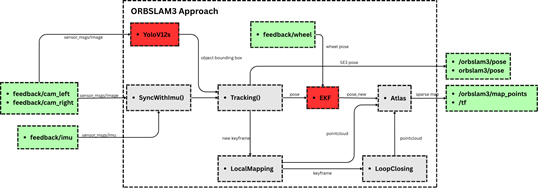
\includegraphics[width=\textwidth]{figures/template/pipeline1_orb.png}
  \caption[Pipeline~1, YOLO26 + ORB-SLAM3, as designed: stereo images and IMU are synchronised, tracked and passed to local mapping, loop closing and the Atlas map; the detector's boxes enter the tracking stage.]{Pipeline~1, YOLO26 + ORB-SLAM3, as designed: stereo images and IMU
  are synchronised, tracked and passed to local mapping, loop closing and the
  Atlas map; the detector's boxes enter the tracking stage. The EKF block that
  fuses the SLAM pose with wheel feedback is a planned integration point and is
  not exercised in this report.}
  \label{fig:pipeline1}
\end{figure}

\begin{figure}[htbp]
  \centering
  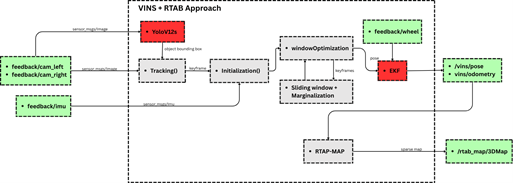
\includegraphics[width=\textwidth]{figures/template/pipeline2_vins_rtab.png}
  \caption[Pipeline~2, YOLO26 + VINS + RTAB-Map, as designed: VINS tracking, initialisation and sliding-window optimisation produce odometry, RTAB-Map builds the map from that odometry and the stereo images.]{Pipeline~2, YOLO26 + VINS + RTAB-Map, as designed: VINS tracking,
  initialisation and sliding-window optimisation produce odometry, RTAB-Map
  builds the map from that odometry and the stereo images. As in
  \cref{fig:pipeline1}, the EKF fusion with wheel feedback is planned.}
  \label{fig:pipeline2}
\end{figure}

\begin{table}[htbp]
\centering
\caption{Design comparison of the two pipeline architectures, as proposed.}
\label{tab:pipeline-comparison}
\small
\begin{tabularx}{\textwidth}{>{\raggedright\arraybackslash}p{0.26\textwidth}>{\raggedright\arraybackslash}X>{\raggedright\arraybackslash}X}
\toprule
Aspect & Pipeline~1: YOLO26 + ORB-SLAM3 & Pipeline~2: YOLO26 + VINS + RTAB-Map \\
\midrule
System structure & tightly coupled (centralised) & decoupled (odometry separate
  from back end) \\
Odometry & ORB-SLAM3 tracking thread; tightly-coupled MAP estimation over
  visual and IMU terms & VINS-Fusion local VIO; sliding-window optimisation \\
Lifelong-mapping mechanism & Atlas multi-map system and map merging
  ($\mathrm{Sim}(3)$) & RTAB-Map memory management (WM / LTM node transfer) \\
Computation-time bound & grows with the number of keyframes and sub-maps in
  Atlas & held at a constant $O(1)$ ceiling in working memory \\
RAM / CPU use & grows with accumulated map size & bounded through the
  processing-time threshold $T_{\max}$ \\
Robustness to vibration & moderate to high; relies on ORB features and IMU
  pre-integration & very high; online temporal and spatial calibration in VINS \\
\bottomrule
\end{tabularx}
\end{table}

\section{The Pipelines as Implemented}
\label{sec:pipelines-implemented}

\subsection{Dynamic feature masking}
\label{sec:masking-formal}

In a dynamic warehouse a conventional SLAM algorithm accumulates drift if it
uses features on moving objects to compute distance. The project therefore
designs a shared front end in which the detector's output filters the geometric
features before they reach the back end. When the stereo camera delivers frame
$I_t$ at time $t$, the image is passed to the YOLO26 network, which returns a
set of bounding boxes
\begin{equation}
  \mathcal{B} = \{B_1, B_2, \ldots, B_K\}, \qquad
  B_k = \{x_k, y_k, w_k, h_k, c_k, P_k\},
  \label{eq:boxes}
\end{equation}
where $(x_k,y_k)$ is the box centre, $(w_k,h_k)$ its width and height, $c_k$
the class label and $P_k$ the confidence. Boxes with $P_k < \tau_{\mathrm{conf}}$
are rejected to limit false positives. Meanwhile the SLAM tracking thread
extracts the frame's feature set $\mathcal{F} = \{f_1,\ldots,f_N\}$ with
$f_i = (u_i, v_i)$. A feature is labelled dynamic when
\begin{equation}
  \exists\, B_k \in \mathcal{B}:\;
  \Bigl(x_k - \tfrac{w_k}{2} \le u_i \le x_k + \tfrac{w_k}{2}\Bigr) \wedge
  \Bigl(y_k - \tfrac{h_k}{2} \le v_i \le y_k + \tfrac{h_k}{2}\Bigr),
  \label{eq:mask-test}
\end{equation}
and is removed immediately, leaving the static feature set
\begin{equation}
  \mathcal{F}_{\mathrm{static}} = \{\, f_i \in \mathcal{F} \mid f_i \notin B_k\ \forall k \,\},
  \label{eq:static-set}
\end{equation}
which is passed to feature matching and re-projection-error minimisation. The
following subsections state where in each estimator that test is actually
applied, because the two front ends re-use features differently and a single
insertion point is not sufficient for both.

\subsection{ORB-SLAM3 and semantic feature rejection}
\label{sec:orb-method}
% Verbatim from minor_report/chapters/chapter_3_methodology.tex lines 1047-1135 (retired report),
% headings demoted by 0 level(s). Do not edit here; edit the source of the numbers.


The project provides a purpose-built ROS~2 Humble wrapper around the pinned
ORB-SLAM3 core. Approximate-time synchronization pairs left and right images with
a \SI{0.02}{\second} slop. Raw and compressed transports are supported. Image
callbacks place stereo pairs in a one-frame queue; a worker thread calls
\texttt{TrackStereo()} so blocking visual tracking does not starve the
\SI{200}{\hertz} IMU subscription. If tracking falls behind, the older pending
image is discarded and the drop count is reported.

With \repo{filter:=false}, no detection subscription is created and an empty mask
passes through the patched interfaces. With filtering enabled, a bounded buffer
is searched for the detection closest in source-image time, accepted only within
\SI{0.15}{\second}. Boxes are expanded by eight pixels, clipped to the image, and
rasterized to an 8-bit mask in which 255 retains a feature and zero rejects it. A
mask covering more than 0.8 of the frame is discarded as a safety measure.

The mask passes through \texttt{System}, \texttt{Tracking}, and \texttt{Frame} to
the ORB extractor. Candidate keypoints are tested before octree distribution, so
the per-level feature quota can be redistributed across surviving static regions.
At each pyramid level, the implemented boundary rule rejects a candidate when at
least five samples in a $3\times3$ neighbourhood are dynamic. Only left-camera
features are masked because ORB-SLAM3 establishes stereo matches from left
keypoints to right candidates.

The current simulation YAML requests \num{1500} ORB features, eight pyramid
levels, a 1.2 scale factor, initial FAST threshold 20, and fallback threshold 7;
\cref{tab:orb-params} collects these. An earlier draft of this section reported
\num{1000} and attributed \num{1500} to a superseded engineering note. That was
backwards: \repo{ORBextractor.nFeatures} is \num{1500} in the committed
configuration, and no uncommitted change touches it. No controlled feature-count
or FAST-threshold sweep is complete.

\begin{figure}[htbp]
  \centering
  \resizebox{\textwidth}{!}{% ORB-SLAM3 pipeline, drawn to show WHERE the semantic mask enters.
% The single point of the figure: the mask is applied to candidate keypoints
% BEFORE octree distribution, which is why the per-level quota can redistribute
% onto surviving static regions. Green is built here, grey is upstream
% ORB-SLAM3, blue-grey is the optional detector path.
\begin{tikzpicture}[
  font=\footnotesize,
  node distance=6mm,
  box/.style={draw, rounded corners, align=center, minimum height=8mm,
    text width=26mm, inner sep=1.6mm, fill=implemented},
  up/.style={box, fill=gray!12},
  det/.style={box, fill=external},
  io/.style={box, fill=gray!5, draw=gray!60},
  flow/.style={-{Latex[length=2mm]}, thick},
  opt/.style={flow, dashed},
  lbl/.style={font=\scriptsize, inner sep=1pt}
]
  % --- inputs
  \node[io]  at (0,   1.5) (stereo) {stereo pair\\\SI{30}{\hertz}};
  \node[io]  at (0,  -1.5) (imu)    {IMU\\\SI{200}{\hertz}};
  \node[det] at (0,   4.2) (yolo)   {YOLO detector\\(optional)};

  % --- wrapper, built here
  \node[box] at (4.2, 1.5) (sync)  {approx-time sync\\\SI{0.02}{\second} slop};
  \node[box] at (8.2, 1.5) (queue) {one-frame queue\\older frame dropped};
  \node[box] at (4.2, 4.2) (match) {nearest-in-time match\\$\le\SI{0.15}{\second}$};
  \node[box] at (8.2, 4.2) (mask)  {expand \SI{8}{px}, clip,\\rasterize 8-bit mask};

  % --- upstream core
  \node[up]  at (12.4, 1.5) (track) {\texttt{TrackStereo()}\\worker thread};
  \node[up]  at (12.4, 4.2) (extr)  {ORB extractor\\candidate keypoints};
  \node[up]  at (16.6, 4.2) (octree){octree\\distribution};
  \node[up]  at (16.6, 1.5) (ba)    {local mapping,\\loop closing};
  \node[io]  at (16.6,-1.5) (out)   {\repo{vio.csv}, TF,\\\repo{/orbslam3/pose}};

  \draw[flow] (stereo) -- (sync);
  \draw[flow] (sync)   -- (queue);
  \draw[flow] (queue)  -- (track);
  \draw[flow] (imu)    -| (track.south);
  \draw[opt]  (yolo)   -- (match);
  \draw[opt]  (match)  -- (mask);
  \draw[flow] (track)  -- (extr);
  \draw[flow] (extr)   -- (octree);
  \draw[flow] (octree) -- (ba);
  \draw[flow] (ba)     -- (out);

  % --- the insertion point, which is the reason the figure exists
  \draw[opt] (mask) -- node[lbl, above=3mm]{mask} (extr);
  \node[draw=flagred, thick, rounded corners, inner sep=2.2mm, fit=(extr)] (hl) {};
  \node[lbl, text=flagred, above=1.5mm of hl]
    {rejected here, \emph{before} distribution};

\end{tikzpicture}
}
  \caption[ORB-SLAM3 pipeline and the semantic-mask insertion point.]{ORB-SLAM3 pipeline and the semantic-mask insertion point. Green is
  built by this project, grey is the pinned upstream core, blue the optional
  detector path. The mask is applied to candidate keypoints \emph{before} octree
  distribution, which is what allows the per-level feature quota to redistribute
  onto surviving static regions rather than simply shrink. A candidate is
  rejected when at least five samples of its $3\times3$ neighbourhood are
  dynamic, and only the left camera is masked, because ORB-SLAM3 forms stereo
  matches outwards from left keypoints.}
  \label{fig:orb-pipeline}
\end{figure}

\begin{table}[htbp]
\centering
\caption[ORB-SLAM3 configuration at the cutoff.]{ORB-SLAM3 configuration at the cutoff. Wrapper values are from
\repo{orbslam3_ros2/src/}; extractor and IMU values from
\repo{config/wil_sim/stereo_imu.yaml}. Noise densities are given in
\cref{tab:imu-noise-assumed} and are not repeated here.}
\label{tab:orb-params}
\small
\setlength{\tabcolsep}{4pt}
\begin{tabularx}{\textwidth}{>{\raggedright\arraybackslash}p{0.30\textwidth}l>{\raggedright\arraybackslash}X}
\toprule
Parameter & Value & Role \\
\midrule
\multicolumn{3}{l}{\emph{Wrapper (built here)}} \\
Stereo sync slop & \SI{0.02}{\second} & approximate-time pairing \\
Image queue depth & 1 frame & older frame dropped, drop count logged \\
Detector match window & \SI{0.15}{\second} & nearest in source-image time \\
Box expansion & \SI{8}{px} & before rasterizing the mask \\
Mask reject threshold & 0.8 of frame & safety cut-out on runaway coverage \\
Boundary rule & $\ge 5$ of $3\times3$ & candidate rejected when dynamic \\
Masked camera & left only & stereo matches form from left keypoints \\
\midrule
\multicolumn{3}{l}{\emph{Extractor and core}} \\
\repo{ORBextractor.nFeatures} & \num{1500} & per-frame feature budget \\
\repo{ORBextractor.nLevels} & 8 & pyramid levels \\
\repo{ORBextractor.scaleFactor} & 1.2 & inter-level scale \\
\repo{ORBextractor.iniThFAST} & 20 & initial corner threshold \\
\repo{ORBextractor.minThFAST} & 7 & fallback threshold \\
\repo{Stereo.ThDepth} & 90.0 & close/far stereo split \\
\repo{IMU.Frequency} & \SI{200}{\hertz} & preintegration rate \\
\repo{loopClosing} & 1 & \flag{comment in the same file says ``set to 0
  deliberately''} \\
\bottomrule
\end{tabularx}
\end{table}

The wrapper publishes \repo{/orbslam3/odometry}, \repo{/orbslam3/pose}, and TF
after valid tracking. It writes the common 11-column trajectory format directly
and flushes each row. Repository evidence is located in
\repo{orbslam3_ros2/src/orbslam3_node.cpp},
\repo{orbslam3_ros2/src/slam_wrapper.cpp},
\repo{orbslam3_ros2/src/trajectory_writer.cpp}, and
\repo{orbslam3_ros2/config/wil_sim/stereo_imu.yaml}.


\subsection{VINS-Fusion front end}
\label{sec:vins-rtab-method}
% Verbatim from minor_report/chapters/chapter_3_methodology.tex lines 1142-1211 (retired report),
% headings demoted by 0 level(s). Do not edit here; edit the source of the numbers.

VINS-Fusion uses stereo features and inertial measurements in a sliding-window
nonlinear estimator. The ROS wrapper synchronizes the raw image topics and uses
separate callback groups for images, IMU, feature messages, and detections. The
simulation configuration processes every image (\repo{image_skip: 1}), uses two
cameras and IMU, fixes simulated extrinsics, targets \SI{25}{\hertz} feature
publication, and uses 10-pixel keyframe parallax. Image queues were increased to
100 and the IMU queue to 2,000 to reduce losses during initialization and backlog.

VINS cannot use only the ORB strategy because it propagates existing features
with pyramidal KLT optical flow and detects new features only for replenishment.
A feature attached to an object before detection could otherwise persist after
masking. The implementation initializes \texttt{FeatureTracker::setMask()} from
the YOLO mask. Tracks in zero-valued regions fail the retention test, while the
same mask is passed to \texttt{goodFeaturesToTrack()} to suppress new points. The
count of persistent tracks removed in dynamic regions is accumulated as a
mechanism diagnostic.

\begin{figure}[htbp]
  \centering
  \resizebox{\textwidth}{!}{% VINS-Fusion pipeline, drawn to show that the mask must act at TWO points.
% The contrast with the ORB figure is the point of both: ORB extracts fresh
% features every frame, so rejecting candidates at extraction is sufficient.
% VINS propagates existing KLT tracks, so suppressing new features alone would
% leave a track that latched onto an object before it was detected still
% attached to it. Both insertions are therefore required.
%
% Layout note: marginalization sits ABOVE the optimizer rather than below it so
% that the IMU can be routed orthogonally beneath the whole diagram. A straight
% IMU-to-optimizer line cuts through goodFeaturesToTrack() and the highlight box.
\begin{tikzpicture}[
  font=\footnotesize,
  box/.style={draw, rounded corners, align=center, minimum height=8mm,
    text width=26mm, inner sep=1.6mm, fill=implemented},
  up/.style={box, fill=gray!12},
  det/.style={box, fill=external},
  ext/.style={box, fill=external},
  io/.style={box, fill=gray!5, draw=gray!60},
  flow/.style={-{Latex[length=2mm]}, thick},
  opt/.style={flow, dashed},
  lbl/.style={font=\scriptsize, inner sep=1pt}
]
  \node[det] at ( 0.0,  4.6) (yolo)   {YOLO detector\\(optional)};
  \node[box, text width=32mm]
             at ( 4.8,  4.6) (setmask){\texttt{FeatureTracker::}\\\texttt{setMask()}};
  \node[up]  at ( 4.8,  2.3) (klt)    {propagate tracks\\pyramidal KLT};
  \node[up]  at ( 4.8,  0.0) (gftt)   {\texttt{goodFeatures}\\\texttt{ToTrack()}};
  \node[io]  at ( 0.0,  1.15)(stereo) {stereo pair\\\SI{30}{\hertz}};
  \node[io]  at ( 0.0, -2.6) (imu)    {IMU\\\SI{200}{\hertz}};
  \node[up]  at ( 9.8,  1.15)(window) {sliding window\\optimization};
  \node[up]  at ( 9.8,  3.8) (marg)   {marginalization};
  \node[io]  at (14.4,  1.15)(out)    {\repo{vio.csv},\\\texttt{world}$\to$\texttt{body}};
  \node[ext] at (14.4, -2.6) (rtab)   {RTAB-Map\\external back end};

  \draw[flow] (stereo.east) -- (klt.west);
  \draw[flow] (stereo.east) -- (gftt.west);
  \draw[flow] (klt.east)    -- (window.west);
  \draw[flow] (gftt.east)   -- (window.west);
  % Orthogonal, beneath everything: nothing sits between y=-2.6 and the
  % optimizer's south face at x=9.8.
  \draw[flow] (imu)         -| (window.south);
  \draw[flow] ([xshift=-4mm]window.north) -- ([xshift=-4mm]marg.south);
  \draw[flow] ([xshift=4mm]marg.south)    -- ([xshift=4mm]window.north);
  \draw[flow] (window)      -- (out);
  \draw[flow] (out)         -- (rtab);
  \draw[opt]  (yolo)        -- (setmask);

  % --- the two insertions, which is the reason the figure exists
  \draw[opt] (setmask) -- (klt);
  \node[lbl, right=1mm] at (4.8, 3.45) {\textbf{1} cull};
  % Down the corridor between the highlight box and the optimizer.
  \draw[opt] (setmask.east) -- (7.3, 4.6) -- (7.3, 0.0) -- (gftt.east);
  \node[lbl, right=1mm] at (7.3, 2.6) {\textbf{2} suppress};
  \node[draw=flagred, thick, rounded corners, inner sep=2.4mm,
        fit=(klt)(gftt)] (hl) {};
  \node[lbl, text=flagred, below=1.5mm of hl] {both insertions required};
\end{tikzpicture}
}
  \caption[VINS-Fusion pipeline and its two semantic-mask insertion points.]{VINS-Fusion pipeline and its two semantic-mask insertion points.
  Because the front end propagates existing KLT tracks and only detects new
  features to replenish them, suppressing new detections alone is insufficient:
  a track that attached to an object before it was detected would survive
  masking. Tracks in masked regions must therefore also be culled (1) while the
  same mask suppresses replenishment (2). Contrast \cref{fig:orb-pipeline},
  where re-extraction every frame makes a single insertion sufficient. The count
  of persistent tracks removed is logged as a mechanism diagnostic --- the
  counter that read zero in all twelve filtered runs.}
  \label{fig:vins-pipeline}
\end{figure}

\begin{table}[htbp]
\centering
\caption[VINS-Fusion simulation configuration at the cutoff, from \repo{vins_fusion_ros2/config/wil_sim/stereo_imu.yaml}.]{VINS-Fusion simulation configuration at the cutoff, from
\repo{vins_fusion_ros2/config/wil_sim/stereo_imu.yaml}. Inertial noise densities
are in \cref{tab:imu-noise-assumed}.}
\label{tab:vins-params}
\small
\setlength{\tabcolsep}{4pt}
\begin{tabularx}{\textwidth}{>{\raggedright\arraybackslash}p{0.26\textwidth}l>{\raggedright\arraybackslash}X}
\toprule
Parameter & Value & Role \\
\midrule
\repo{num_of_cam} / \repo{imu} & 2 / 1 & stereo-inertial \\
\repo{image_skip} & 1 & every image processed \\
\repo{max_cnt} & 150 & tracked-feature budget \\
\repo{min_dist} & \SI{30}{px} & minimum feature separation \\
\repo{freq} & \SI{25}{\hertz} & target feature publication \\
\repo{keyframe_parallax} & \SI{10}{px} & keyframe decision \\
\repo{F_threshold} & 1.0 & RANSAC fundamental-matrix gate \\
\repo{max_solver_time} & \SI{0.08}{\second} & Ceres budget per update \\
\repo{max_num_iterations} & 100 & Ceres iteration cap \\
\repo{estimate_extrinsic} & 0 & simulated extrinsics held fixed \\
\repo{estimate_td} & 0 & camera--IMU delay held at \SI{0}{\second} \\
\repo{g_norm} & \SI{9.8}{\metre\per\second\squared} & matches the world's gravity \\
Image queue & 100 & raised to survive initialization backlog \\
IMU queue & \num{2000} & raised for the same reason \\
\bottomrule
\end{tabularx}
\end{table}

VINS writes the optimized state after each estimator update to \repo{vio.csv} and
broadcasts \texttt{world~$\rightarrow$~body} using configurable frame names. The
ROS \repo{output_path} parameter overrides the YAML path, recursively creates
missing directories, and reports an explicit error if \repo{vio.csv} cannot be
opened. This behaviour is an uncommitted worktree change at the cutoff. Evidence
is in \repo{vins_fusion_ros2/src/vins_estimator.cpp},
\repo{vins_fusion_ros2/vins/src/featureTracker/feature_tracker.cpp}, and
\repo{vins_fusion_ros2/vins/src/estimator/estimator.cpp}.


\subsection{RTAB-Map mapping and localization back end}
\label{sec:rtab-method}
% Verbatim from minor_report/chapters/chapter_3_methodology.tex lines 1215-1258 (retired report),
% headings demoted by 0 level(s). Do not edit here; edit the source of the numbers.

RTAB-Map receives front-end odometry through TF and stereo imagery through
\repo{rtab_camera_shim.py}. The shim reconstructs \texttt{CameraInfo}, decompresses
the pair, and publishes validated static camera transforms from the common
simulation calibration. TF was selected over an odometry topic because adding
high-rate odometry to multi-topic approximate synchronization starved the
lower-rate images. The cost is that odometry covariance is not supplied to graph
edge weighting.

The back end uses stereo SGBM (\repo{Stereo/DenseStrategy: 1}), height-based
ground separation, ray tracing, spatial noise filtering, and odometry-derived
gravity links. Its measured default depth range is \SI{10}{\metre}. Because the
featureless floor provides essentially no stereo ground points, ray tracing
supplies free-space evidence between the sensor and observed obstacles. These
settings affect occupancy assembly; visual-word loop closure is separate.

Three modes are provided by one launch file:
\begin{description}
  \item[construct] starts a new incremental database;
  \item[extend] opens an existing database, places prior nodes in working memory,
    and permits new nodes; and
  \item[localize] disables incremental memory, loads existing nodes, serves the
    saved map, and can enable \repo{Mem/LocalizationReadOnly}.
\end{description}

Localization still extracts features from current stereo images and matches
stored RTAB-Map signatures. Read-only mode prevents database modification; it
does not disable perception. The outputs are an external
\texttt{map~$\rightarrow$~odom} correction and \repo{/localization_pose}. Neither
RTAB-Map features nor corrected poses are injected into ORB-SLAM3's Atlas or
VINS-Fusion's sliding window.

The composed localization launch raises \repo{RGBD/OptimizeMaxError} from 3.0 to
10.0 because the default rejected all loop closures proposed with the observed
VINS drift. This is effective operationally but is not yet proven safe against
perceptual aliasing in repeated warehouse bays. Occupancy creation is disabled in
localization mode because the stored map is reused. Live VINS-Fusion and RTAB-Map
co-execution nevertheless remains blocked on the current machine. Recorded
\repo{vio.csv} can be replayed as \texttt{odom~$\rightarrow$~vio\_body} for a
deterministic back-end test, but this is not proof of real-time co-execution.

Evidence is in \repo{rtabmap_ros/rtab_sim.launch.py},
\repo{rtabmap_ros/rtab_camera_shim.py},
\repo{aws-robomaker-small-warehouse-world/launch/localization_rtabmap.launch.py},
and \repo{script/gt_tf_publisher.py}.


\subsection{YOLO detector node, mask construction and synchronisation}
\label{sec:yolo-method}
% Verbatim from minor_report/chapters/chapter_3_methodology.tex lines 1483-1516 (retired report),
% headings demoted by 0 level(s). Do not edit here; edit the source of the numbers.

The semantic front end is a standalone Python ROS~2 node using Ultralytics. The
project checkpoint is \repo{weight/best.pt}, a custom detector for \texttt{bin},
\texttt{box}, and \texttt{bucket}, fine-tuned from \repo{yolo26m.pt} using
640-pixel inputs. It produces bounding boxes, not segmentation masks. The stock
\repo{yolo26n.pt} and \repo{yolo26m.pt} files are not project-trained models and
are not evidence of custom training.

At startup, the node resolves requested classes against checkpoint metadata,
warms the model with three dummy images, and selects CUDA when available. Current
defaults are confidence 0.35, NMS IoU 0.5, and image size 640. Only the left image
is processed. Each \texttt{Detection2DArray} preserves the source image header,
so nearest-timestamp selection measures sensor-time correspondence rather than
inference-completion time. Empty arrays distinguish a valid frame with no
detections from detector failure.

The detector intentionally remains outside stereo synchronization. A three-input
image/image/detection synchronizer would discard pairs whenever inference lagged.
The implemented design continues without filtering if no recent detection exists.
Filtered runs write \repo{yolo_mask.csv} with timestamp, box count, coverage,
match state, detection age, and rejection status.

Offline evaluation in \repo{script/yolo_eval.py} transforms Gazebo model poses and
collision-mesh vertices into the left-camera frame to form projected truth boxes.
Object speed over \SI{0.05}{\metre\per\second} defines the moving subset.
Predictions are greedily matched by class at IoU 0.5. Heavily occluded truth boxes
and predictions covered by known but unlabeled box-like scenery are ignored at
stated thresholds. Outputs are per-frame \repo{yolo_eval.csv}, per-detection
\repo{yolo_detections.csv}, and overlays. Overlays are inspected before aggregate
metrics because invalid pose stamps, centimetre mesh units, or malformed camera
transforms can produce plausible but invalid numbers.

The current semantic rule assumes all selected-class detections are dynamic. No
optical-flow, stereo-depth, or world-motion gate is implemented, and axis-aligned
boxes also remove background pixels. These are explicit method limitations.


\section{Simulation Platform}
\label{sec:sim-platform}

\subsection{Computing and software environment}
% Verbatim from minor_report/chapters/chapter_3_methodology.tex lines 108-160 (retired report),
% headings demoted by 0 level(s). Do not edit here; edit the source of the numbers.

One machine produced every simulation result in this report.
\Cref{tab:compute-environment} records it. Each entry was re-read from the
running system on 20 September 2026 rather than copied forward from the
engineering log, and all agreed.

\begin{table}[htbp]
\centering
\caption[Computing and software environment.]{Computing and software environment. A single laptop produced every
result reported here; there is no second platform, so no entry below supports a
cross-hardware comparison.}
\label{tab:compute-environment}
\small
\setlength{\tabcolsep}{4pt}
\begin{tabularx}{\textwidth}{>{\raggedright\arraybackslash}p{0.20\textwidth}>{\raggedright\arraybackslash}p{0.30\textwidth}>{\raggedright\arraybackslash}X}
\toprule
Component & Version & Role \\
\midrule
\multicolumn{3}{l}{\emph{Platform}} \\
Operating system & Ubuntu 22.04.5 LTS & \\
Middleware & ROS~2 Humble & \\
CPU & 16 logical cores & \\
Memory & \SI{15}{\giga\byte}, no swap & no swap, so memory pressure fails
  outright rather than degrading \\
GPU & NVIDIA RTX~3070 Laptop & detector inference only \\
\midrule
\multicolumn{3}{l}{\emph{Build toolchain}} \\
GCC & 11.4.0 & \\
CMake & 3.22.1 & \\
OpenCV (system) & 4.5.4 & links both estimators \\
Pangolin & 0.9.1 & ORB-SLAM3 built out of tree \\
\midrule
\multicolumn{3}{l}{\emph{Detector environment}} \\
PyTorch & 2.5.1+cu121 & \\
torchvision & 0.20.1+cu121 & \\
Ultralytics & 8.4.138 & YOLO training and inference \\
NumPy & 1.26.4 & \\
OpenCV (Python) & 4.11.0 & \flag{differs from the 4.5.4 the estimators link} \\
\midrule
\multicolumn{3}{l}{\emph{Mapping back end}} \\
\repo{ros-humble-rtabmap} & 0.23.7 & apt core library \\
RTAB-Map ROS wrappers & project checkout & only packages through
  \repo{rtabmap_slam} are built \\
\bottomrule
\end{tabularx}
\end{table}

Two consequences follow from the table rather than from any experiment. The
proposed Jetson-versus-laptop study has not been instrumented or executed, so
every timing, throughput and CPU figure in \cref{chap:results} describes this
machine alone and none supports a hardware comparison. And the detector runs a
different OpenCV build from the one the estimators link against, which is
unremarkable for two separate processes but would matter if image handling were
ever moved across that boundary.


\subsection{Simulated sensor rig and platform}
% Verbatim from minor_report/chapters/chapter_3_methodology.tex lines 164-298 (retired report),
% headings demoted by 0 level(s). Do not edit here; edit the source of the numbers.

The simulated Ackermann robot carries two ideal pinhole cameras and an IMU on a
forward mast, and is driven through a front-steering, rear-driven four-wheel
chassis. \Cref{fig:ackermann-robot} gives its dimensioned plan and elevation, and
\cref{tab:sim-sensor-rig,tab:platform-geometry} list the sensor and platform
constants. Every value in the figure and both tables is read from
\repo{aws-robomaker-small-warehouse-world/models/ackermann_robot/model.sdf}, so
the drawing is to scale rather than illustrative.

\begin{figure}[htbp]
  \centering
  \resizebox{\textwidth}{!}{% Dimensioned plan and elevation of the simulated Ackermann robot.
%
% Every coordinate below is read from
% aws-robomaker-small-warehouse-world/models/ackermann_robot/model.sdf and is
% expressed in metres relative to base_footprint, so the drawing is to scale and
% can be re-derived from the model rather than trusted. A Gazebo screenshot was
% deliberately not used: the quantities that matter to the estimators are the
% wheel base, track, wheel radius and sensor offsets, and a perspective render
% shows none of them.
%
% NOTE ON THE TWO VIEWS. They are placed side by side with shift={(1.45,0)},
% i.e. in DIAGRAM units, not with yshift/xshift in centimetres. Inside a scope
% that already carries scale=9 a shift given in cm is multiplied by that scale,
% which silently pushes the second view about 56 cm away and off the page.
\begin{tikzpicture}[
  scale=9,
  chassis/.style={draw, fill=gray!12, thick},
  wheel/.style={draw, fill=gray!45, thick},
  steered/.style={draw, dashed, gray!60!black, line width=0.4pt},
  mast/.style={draw, fill=gray!25},
  sensor/.style={draw, fill=external, thick},
  imu/.style={draw, fill=implemented, thick},
  dim/.style={{Latex[length=1.2mm]}-{Latex[length=1.2mm]}, gray!60!black,
    line width=0.3pt},
  dimlab/.style={font=\tiny, inner sep=1pt, fill=white},
  leader/.style={gray!60!black, line width=0.25pt},
  lbl/.style={font=\tiny, inner sep=1pt},
  tick/.style={gray!60!black, line width=0.25pt}
]

% ======================= PLAN VIEW (x forward, y left) =======================
\begin{scope}
  \node[font=\small\bfseries] at (0.15,0.44) {Plan view};

  % chassis deck: 0.6 x 0.463 centred on base_footprint
  \draw[chassis] (-0.3,-0.2315) rectangle (0.3,0.2315);

  % steered front wheels shown at full lock, +/-0.6109 rad = +/-35 deg,
  % rotated about the kingpin rather than drawn as a bare angle sweep
  \foreach \y in {0.21,-0.21}{
    \begin{scope}[shift={(0.21,\y)}, rotate=35]
      \draw[steered] (-0.0585,-0.0325) rectangle (0.0585,0.0325);
    \end{scope}
  }

  % wheels: radius 0.0585, half-width 0.0325, at x = +/-0.21, y = +/-0.21
  \foreach \x in {0.21,-0.21}{
    \foreach \y in {0.21,-0.21}{
      \draw[wheel] (\x-0.0585,\y-0.0325) rectangle (\x+0.0585,\y+0.0325);
    }
  }
  \node[lbl, anchor=south west] at (0.135,0.275)
    {$\delta_{\max}=\pm\SI{0.6109}{\radian}$};

  % camera mast and the two cameras
  \draw[mast] (0.3078,-0.01) rectangle (0.5395,0.01);
  \draw[sensor] (0.486,0.0836) rectangle (0.506,0.1036);
  \draw[sensor] (0.486,-0.01) rectangle (0.506,0.01);

  % IMU
  \draw[imu] (0.313,-0.025) rectangle (0.363,0.025);
  \node[lbl, anchor=north] at (0.338,-0.032) {\texttt{imu}};

  % base_footprint origin marker
  \draw[thick] (-0.025,0) -- (0.025,0) (0,-0.025) -- (0,0.025);
  \node[lbl, anchor=north] at (0,-0.035) {\texttt{base\_footprint}};

  % camera labels, lifted clear on leaders so they cannot collide with the
  % baseline dimension between them
  \draw[leader] (0.506,0.0936) -- (0.60,0.155);
  \node[lbl, anchor=west] at (0.605,0.155) {\texttt{cam0} (left)};
  \draw[leader] (0.506,0) -- (0.60,-0.075);
  \node[lbl, anchor=west] at (0.605,-0.075) {\texttt{cam1} (right)};

  % --- dimensions ---
  \draw[tick] (0.21,-0.2425) -- (0.21,-0.315);
  \draw[tick] (-0.21,-0.2425) -- (-0.21,-0.315);
  \draw[dim] (-0.21,-0.30) -- (0.21,-0.30);
  \node[dimlab] at (0,-0.30) {wheel base \SI{0.42}{\metre}};

  \draw[tick] (-0.2685,0.21) -- (-0.375,0.21);
  \draw[tick] (-0.2685,-0.21) -- (-0.375,-0.21);
  \draw[dim] (-0.36,-0.21) -- (-0.36,0.21);
  \node[dimlab, rotate=90] at (-0.36,0) {track \SI{0.42}{\metre}};

  \draw[tick] (0.506,0.0936) -- (0.565,0.0936);
  \draw[tick] (0.506,0) -- (0.565,0);
  \draw[dim] (0.552,0) -- (0.552,0.0936);
  \node[dimlab, rotate=90] at (0.552,0.047) {\SI{0.0936}{\metre}};
\end{scope}

% ======================= ELEVATION (x forward, z up) =======================
\begin{scope}[shift={(1.45,-0.16)}]
  \node[font=\small\bfseries] at (0.15,0.60) {Side elevation};

  % ground line
  \draw[gray!55, line width=0.5pt] (-0.38,0) -- (0.60,0);

  % wheels seen edge on: centre z = 0.072, radius 0.0585
  \foreach \x in {0.21,-0.21}{
    \draw[wheel] (\x,0.072) circle (0.0585);
    \draw[gray!60!black, line width=0.25pt] (\x,0.072) circle (0.007);
  }

  % chassis deck: z from 0.072 to 0.122
  \draw[chassis] (-0.3,0.072) rectangle (0.3,0.122);

  % mast: vertical post, camera bar, short riser
  \draw[mast] (0.399,0.122) rectangle (0.419,0.3715);
  \draw[mast] (0.3078,0.3715) rectangle (0.5395,0.3915);
  \draw[mast] (0.486,0.3915) rectangle (0.506,0.4295);

  % cameras at z = 0.4395 (cam0 hides cam1 in this projection)
  \draw[sensor] (0.482,0.4295) rectangle (0.510,0.4495);
  \draw[leader] (0.510,0.4395) -- (0.55,0.50);
  \node[lbl, anchor=west] at (0.555,0.50) {\texttt{cam0}, \texttt{cam1}};

  % IMU at z = 0.192
  \draw[imu] (0.313,0.182) rectangle (0.363,0.202);
  \draw[leader] (0.363,0.192) -- (0.44,0.25);
  \node[lbl, anchor=west] at (0.445,0.25) {\texttt{imu}, $z=\SI{0.192}{\metre}$};

  % --- dimensions ---
  \draw[dim] (0.21,0.072) -- (0.21,0.1305);
  \node[dimlab, anchor=west] at (0.222,0.101) {$r=\SI{0.0585}{\metre}$};

  \draw[tick] (0.510,0.4395) -- (0.585,0.4395);
  \draw[dim] (0.572,0) -- (0.572,0.4395);
  \node[dimlab, rotate=90] at (0.572,0.22) {\SI{0.4395}{\metre}};

  \draw[tick] (-0.2685,0.072) -- (-0.375,0.072);
  \draw[dim] (-0.36,0) -- (-0.36,0.072);
  \node[dimlab, rotate=90] at (-0.36,0.036) {axle \SI{0.072}{\metre}};
\end{scope}

\end{tikzpicture}
}
  \caption[Simulated Ackermann platform, drawn to scale from the model definition.]{Simulated Ackermann platform, drawn to scale from the model
  definition. Distances are in metres relative to \texttt{base\_footprint}. The
  stereo pair is mounted asymmetrically: \texttt{cam1} sits on the vehicle
  centreline and \texttt{cam0} is offset \SI{0.0936}{\metre} to its left, so the
  optical centre of the pair is not the chassis centreline. The wheel base and
  track are equal at \SI{0.42}{\metre}, which is what makes the rear-wheel
  differential a poor yaw-rate estimator (\cref{sec:proprio-method}).}
  \label{fig:ackermann-robot}
\end{figure}

\begin{table}[htbp]
\centering
\caption[Simulated sensor configuration.]{Simulated sensor configuration. Intrinsics are analytic rather than
calibrated: the simulator renders an exact pinhole camera, so $f_x=f_y$ follow
from the image width and the horizontal field of view and the distortion
coefficients are identically zero. The stereo baseline was independently checked
from positive disparity in a recorded bag rather than taken from the model alone.}
\label{tab:sim-sensor-rig}
\small
\resizebox{\textwidth}{!}{%
\begin{tabular}{llll}
\toprule
Quantity & \texttt{cam0} (left) & \texttt{cam1} (right) & \texttt{imu} \\
\midrule
Resolution & $1280\times720$ & $1280\times720$ & -- \\
Rate & \SI{30}{\hertz} & \SI{30}{\hertz} & \SI{200}{\hertz} \\
Horizontal FOV & $\pi/2$ rad (\SI{90}{\degree}) & $\pi/2$ rad (\SI{90}{\degree}) & -- \\
$f_x=f_y$ & 640 & 640 & -- \\
$(c_x,c_y)$ & $(640,360)$ & $(640,360)$ & -- \\
Distortion & zero & zero & -- \\
Position from \texttt{base\_footprint} (m) & $(0.496,0.0936,0.4395)$ &
  $(0.496,0,0.4395)$ & $(0.338,0,0.192)$ \\
Position from IMU body (m) & $(0.158,0.0936,0.2475)$ & $(0.158,0,0.2475)$ &
  $(0,0,0)$ \\
Stereo baseline & \multicolumn{2}{l}{\SI{0.0936}{\metre}} & -- \\
\bottomrule
\end{tabular}}
\end{table}

The fixed camera rotation converts the ROS body convention (forward, left, up) to
the optical convention (right, down, forward). The VINS simulation configuration
fixes the extrinsics (\repo{estimate_extrinsic: 0}) and disables temporal-offset
estimation (\repo{estimate_td: 0}); the assumed inertial noise model is given in
\cref{tab:imu-noise-assumed}, and the same values are mapped to the ORB-SLAM3
configuration.

\begin{table}[htbp]
\centering
\caption[Inertial noise parameters supplied to the visual-inertial estimators, beside the values measured from the recorded IMU stream in \cref{sec:proprio-method}.]{Inertial noise parameters supplied to the visual-inertial estimators,
beside the values measured from the recorded IMU stream in
\cref{sec:proprio-method}. The configured values are inherited estimator defaults,
not measurements of this simulated IMU; the discrepancy is carried forward as a
queried item rather than silently reconciled.}
\label{tab:imu-noise-assumed}
\small
\begin{tabular}{llll}
\toprule
Parameter & Configured (VINS, ORB) & Measured from bag & Units \\
\midrule
\texttt{acc\_n} & 0.02 & \flag{0.0139--0.0294} &
  m\,s$^{-2}/\sqrt{\mathrm{Hz}}$ \\
\texttt{gyr\_n} & 0.002 & \flag{0.000300--0.000364} &
  rad\,s$^{-1}/\sqrt{\mathrm{Hz}}$ \\
\texttt{acc\_w} & 0.001 & not measurable & m\,s$^{-3}/\sqrt{\mathrm{Hz}}$ \\
\texttt{gyr\_w} & 0.0001 & not measurable &
  rad\,s$^{-2}/\sqrt{\mathrm{Hz}}$ \\
\bottomrule
\end{tabular}
\end{table}

\begin{queried}[Queried]
The configured gyroscope noise density is \num{2e-3} whereas the stationary
windows of the five recorded streams give \numrange{3.00e-4}{3.64e-4}, so the
configured value is about six times too large. The configured accelerometer
density of 0.02 sits inside the measured spread but that spread is itself wide,
\numrange{0.0139}{0.0294} across five bags of the same simulated sensor. Both
estimators are therefore running on an inertial noise model that does not
describe this IMU closely. The bias random walks cannot be checked at all: the
longest stationary interval in any \repo{dataset_allsensor} bag is
\SI{1.54}{\second} and an Allan-variance estimate needs minutes. No conclusion in
this report depends on these four numbers, but they should be re-derived from a
dedicated stationary recording before any tuning claim is made.
\end{queried}

\begin{queried}[Queried]
The accelerometer characterisation is not stable across recordings of the same
simulated sensor. \repo{allsensor_002}, whose stationary window is
\SI{1.54}{\second} and therefore the best conditioned of the three, returns an $x$
bias of \SI{0.0683}{\metre\per\second\squared}, against 0.0191 for
\repo{allsensor_000} and \SI{0.0016}{\metre\per\second\squared} for
\repo{allsensor_004}, whose window is the shortest at \SI{0.52}{\second}. The
scale ranges from 1.0199 to 1.0669 over the five. Because the window is short in
every case, part of this spread is estimator variance rather than a property of
the sensor, and the accelerometer terms should not be quoted as calibrated
constants. The gyroscope scale agrees to four decimal places across all five bags;
its bias does not, varying by a factor of twenty, which is consistent with the
same window-length problem.
\end{queried}

\begin{table}[htbp]
\centering
\caption[Platform geometry and drivetrain limits used by the wheel-odometry and EKF baselines.]{Platform geometry and drivetrain limits used by the wheel-odometry and
EKF baselines. \texttt{AckermannSteering} exposes no noise parameter, so the
simulated encoders and odometry are noise free at source.}
\label{tab:platform-geometry}
\small
\begin{tabular}{llll}
\toprule
Quantity & Symbol & Value & Source field \\
\midrule
Wheel base (front to rear axle) & $L$ & \SI{0.42}{\metre} & \texttt{wheel\_base} \\
Track (wheel separation) & $B$ & \SI{0.42}{\metre} & \texttt{wheel\_separation} \\
Kingpin width & -- & \SI{0.42}{\metre} & \texttt{kingpin\_width} \\
Wheel radius & $r$ & \SI{0.0585}{\metre} & \texttt{wheel\_radius} \\
Wheel width & -- & \SI{0.065}{\metre} & wheel \texttt{<length>} \\
Steering limit & $\delta_{\max}$ & $\pm\SI{0.6109}{\radian}$ & \texttt{steering\_limit} \\
Chassis mass & -- & \SI{10.1}{\kilogram} & \texttt{base\_footprint} \texttt{<mass>} \\
Maximum speed & -- & \SI{10}{\metre\per\second} & \texttt{max\_velocity} \\
Maximum acceleration & -- & \SI{3}{\metre\per\second\squared} & \texttt{max\_acceleration} \\
Odometry publish rate & -- & \SI{50}{\hertz} & \texttt{odom\_publish\_frequency} \\
Joint-state publish rate & -- & \SI{1}{\kilo\hertz} & measured from bag \\
\bottomrule
\end{tabular}
\end{table}


\subsection{Simulation fidelity and its limits}
\label{sec:sim-fidelity}
% Verbatim from minor_report/chapters/chapter_3_methodology.tex lines 303-530 (retired report),
% headings demoted by 0 level(s). Do not edit here; edit the source of the numbers.

Every simulation result in this report rests on how faithfully the simulator
reproduces the sensors and the contact physics. This subsection states what is
modelled, what is idealised, and in which direction each idealisation biases the
comparison between the visual and proprioceptive estimators.

\paragraph{Inertial measurement.} \Cref{tab:imu-noise-assumed} reports the noise
measured from the recorded stream and queries it, because no
\repo{dataset_allsensor} bag contains a stationary interval long enough for a
sound estimate. That query can be closed without a new recording: the noise is
\emph{declared}, not emergent, so the simulator's own configuration is the
ground truth the measurement was trying to recover.

\Cref{tab:injected-noise} collects what the simulator actually injects, together
with the measured values and the EuRoC reference. The measured gyroscope range
brackets the declared value, which corroborates both. The measured accelerometer
range does not: it is three to seven times the declared figure, and that
discrepancy is the estimator's rather than the sensor's, because the residual on
the driving axis carries real longitudinal acceleration that a
\SI{1.54}{\second} window cannot separate from noise. Prefer the declared values
wherever a number is needed.

\begin{table}[htbp]
\centering
\caption[Noise injected by the simulator, from the \repo{<imu>} and \repo{<camera>} sensor blocks of the robot model.]{Noise injected by the simulator, from the \repo{<imu>} and
\repo{<camera>} sensor blocks of the robot model. Densities are per-sample
$\sigma$ divided by $\sqrt{f_s}$ at \SI{200}{\hertz}, in the channel's own units
per $\sqrt{\si{\hertz}}$. The EuRoC column is the ADIS16448 of that
benchmark, on which both visual estimators were published.}
\label{tab:injected-noise}
\small
\setlength{\tabcolsep}{4pt}
\begin{tabularx}{\textwidth}{>{\raggedright\arraybackslash}X llll}
\toprule
Channel (units of $\sigma$) & Declared $\sigma$ & Density & Measured & EuRoC \\
\midrule
Gyroscope, per axis (\si{\radian\per\second}) & \num{0.0048} & \num{3.394e-4} &
  \numrange{3.00e-4}{3.64e-4} & \num{1.70e-4} \\
Accelerometer, per axis (\si{\metre\per\second\squared}) & \num{0.0566} &
  \num{4.002e-3} & \flag{\numrange{1.39e-2}{2.94e-2}} & \num{2.00e-3} \\
Camera, per pixel (normalised intensity) & \num{0.005} & --- & not measured & --- \\
\midrule
\multicolumn{5}{l}{\emph{Bias, first-order Gauss--Markov: $\sigma_b$ and
  correlation time $\tau$}} \\
Gyroscope bias (\si{\radian\per\second}) & \num{3.8785e-5} &
  $\tau=\SI{1000}{\second}$ & not measurable & --- \\
Accelerometer bias (\si{\metre\per\second\squared}) & \num{0.006} &
  $\tau=\SI{300}{\second}$ & not measurable & --- \\
\bottomrule
\end{tabularx}
\end{table}

Two readings follow. The simulated IMU is \emph{twice as noisy} as the EuRoC
reference on both channels, so it is not an optimistic sensor. The camera, at
about \num{1.3} grey levels out of \num{255} and with no distortion terms, is
very much cleaner than any real one. Both bias correlation times exceed the
\SIrange{85}{130}{\second} run lengths, so within a run the bias behaves as a
slowly varying constant and its instability is never exercised.

The IMU is therefore not optimistic in its noise. Three things are nonetheless
absent: chassis vibration, which on a real platform is frequently the dominant
error; scale-factor, cross-axis and $g$-sensitivity errors; and temperature
drift. The correlation times also exceed the \SIrange{85}{130}{\second} run
lengths, so within a run the bias behaves as a slowly varying constant and its
instability is never exercised. Finally, the message's \repo{orientation} field
carries no noise block at all and is therefore ground truth; no estimator in this
project consumes it, and none should.

\paragraph{Wheel encoders.} \repo{JointStatePublisher} reports the true solver
angle. Slip consequently appears as a \emph{discrepancy} rather than an error ---
the joint angle stays true, so encoder-integrated distance over-reads whenever
traction breaks, which is exactly a real encoder's behaviour. What is idealised
is resolution: a physical 1024\,CPR encoder quantises to \SI{6.1e-3}{\radian},
setting a floor on low-speed velocity estimation that the simulation does not
have. \repo{script/encoder_sim.py} exists to impose that floor downstream and has
not been applied to any result in this report.

\paragraph{Physics engine and solver.} \Cref{tab:physics-setup} records the
simulation's physics configuration, which is identical across all 26 world files.
Two entries deserve comment because they are easy to misread.

The \repo{<physics>} element declares \repo{type="ignored"}. That is not a
misconfiguration: in Gazebo Fortress the engine is selected by the physics system
plugin, not by that attribute, and the attribute is disregarded. No world passes
an \repo{<engine>} parameter to the plugin, so the engine is Fortress's default,
\repo{dartsim}. This matters for the friction discussion below, and it is the
reason \repo{slip1} and \repo{slip2} have no effect.

No solver block is declared anywhere --- no iteration count, no SOR parameter, no
constraint-force mixing or error-reduction terms. Every one of those therefore
takes the engine default. A \SI{1}{\milli\second} step is a fine integration
step for a \SI{1.4}{\metre\per\second} ground vehicle, but the untuned contact
solver is the part of this setup least able to support a quantitative claim about
contact behaviour.

\begin{table}[htbp]
\centering
\caption[Gazebo physics configuration, identical in all 26 world files.]{Gazebo physics configuration, identical in all 26 world files. Entries
marked ``engine default'' are not declared anywhere in the project and are
therefore whatever \repo{dartsim} chooses.}
\label{tab:physics-setup}
\small
\setlength{\tabcolsep}{4pt}
\begin{tabularx}{\textwidth}{>{\raggedright\arraybackslash}p{0.24\textwidth}>{\raggedright\arraybackslash}p{0.22\textwidth}>{\raggedright\arraybackslash}X}
\toprule
Setting & Value & Note \\
\midrule
Engine & \repo{dartsim} & Fortress default; no world sets \repo{<engine>} \\
\repo{<physics type>} & \repo{"ignored"} & disregarded in Fortress; the plugin
  selects the engine \\
\repo{max_step_size} & \SI{1}{\milli\second} & \SI{1}{\kilo\hertz} integration \\
\repo{real_time_factor} & 1 & no deliberate slow-down \\
\repo{real_time_update_rate} & engine default & not declared \\
Solver type and iterations & engine default & no \repo{<solver>} block anywhere \\
CFM / ERP & engine default & no \repo{<constraints>} block anywhere \\
Gravity & \SI{-9.8}{\metre\per\second\squared} & against ORB-SLAM3's hard-coded
  \num{9.81}, a \SI{0.1}{\percent} difference \\
\repo{slip1}, \repo{slip2} & 0 on all grounds & \flag{an ODE feature;
  \repo{dartsim} does not implement it, so inert at any value} \\
\bottomrule
\end{tabularx}
\end{table}

Achieved real-time factor was not logged during recording, so the table states
the requested factor rather than the realised one. Replay rate, which is logged,
is a separate control and is given per experiment in \cref{chap:results}.

\paragraph{Contact friction, and why the encoder is flattered.} The wheels
declare $\mu=1$, $\mu_2=1$ and every ground model declares $\mu=100$, $\mu_2=50$.
Both sets sit inside \repo{<friction><ode>} elements, which is where SDF places
them irrespective of engine, and \repo{dartsim} consumes them
(\cref{tab:physics-setup}). How it combines two differing coefficients is not
established here, so the effective value is not asserted; what is measured is the
outcome in \cref{tab:measured-slip}.

\repo{slip1} and \repo{slip2} are pinned at zero on all three ground models, but
that is not why force-dependent slip is absent. Those parameters are an ODE
feature, and \repo{dartsim} does not implement them, so they would be inert at
any value. Contact is rigid until Coulomb traction is exceeded regardless.

\Cref{tab:measured-slip} gives the consequence, measured rather than assumed, by
integrating rear-wheel angle against true path length.

\begin{table}[htbp]
\centering
\caption[Measured wheel slip on the five multi-sensor recordings.]{Measured wheel slip on the five multi-sensor recordings. The ratio is
encoder-integrated distance over true path length; above one is slip, below one
is a rolling-radius error and cannot be slip. Measured by
\repo{script/check_slip.py}.}
\label{tab:measured-slip}
\small
\begin{tabular}{lrrr}
\toprule
Recording & Encoder (m) & Truth (m) & Ratio \\
\midrule
\repo{allsensor_000} & 117.12 & 117.05 & 1.0006 \\
\repo{allsensor_001} & 112.91 & 113.11 & 0.9982 \\
\repo{allsensor_002} & 115.37 & 115.20 & 1.0015 \\
\repo{allsensor_003} & 141.68 & 140.61 & 1.0076 \\
\repo{allsensor_004} & 142.36 & 142.25 & 1.0008 \\
\bottomrule
\end{tabular}
\end{table}

Slip is present but under \SI{1}{\percent} everywhere, and on
\repo{allsensor_001} the encoder under-reads, which cannot be slip. Against a
wheel-odometry drift of \SIrange{2.15}{6.57}{\percent}, slip is therefore not the
dominant error; the yaw-rate geometry is, as the falsification of H1 establishes.

\begin{queried}[Threat to validity]
This is a bias with a known direction. The EKF baseline of
\cref{sec:results-proprio} is evaluated on a floor where the wheels effectively
cannot slip and with an encoder of unlimited resolution, which is dead
reckoning's best case. Both idealisations favour the EKF over the visual
estimators, and neither has been relaxed. The conclusion that a wheel+IMU filter
outperforms both visual pipelines should be read as holding \emph{under these
conditions}, not as a general result. \repo{script/make_slippery_floor.py}
generates ground models at a chosen friction coefficient so that traction can be
made an experimental factor; \repo{script/encoder_sim.py} imposes a realistic
quantisation floor. Neither has been used in any result reported here.
\end{queried}

\paragraph{Noise models supplied to the estimators.} The two are not told the
truth about the IMU, as \cref{tab:configured-vs-injected} shows.

\begin{table}[htbp]
\centering
\caption[What the visual estimators are configured to expect, against what the simulator injects.]{What the visual estimators are configured to expect, against what the
simulator injects. Both estimators use identical values. Inflating noise above
datasheet figures is standard practice in visual-inertial odometry and the
configuration records that intent; the ratios are given so the size of the
margin is visible.}
\label{tab:configured-vs-injected}
\small
\begin{tabularx}{\textwidth}{llll>{\raggedright\arraybackslash}X}
\toprule
Parameter & Configured & Injected & Ratio & Quantity \\
\midrule
\repo{gyr_n} & \num{0.002}  & \num{3.394e-4} & \num{5.9}$\times$ &
  gyroscope noise density \\
\repo{acc_n} & \num{0.02}   & \num{4.002e-3} & \num{5.0}$\times$ &
  accelerometer noise density \\
\repo{gyr_w} & \num{0.0001} & \num{1.735e-6} & \flag{\num{58}$\times$} &
  gyroscope bias random walk \\
\repo{acc_w} & \num{0.001}  & \num{4.899e-4} & \num{2.0}$\times$ &
  accelerometer bias random walk \\
\bottomrule
\end{tabularx}
\end{table}

The injected bias random walks are the Gauss--Markov driving densities
$\sigma_b\sqrt{2/\tau}$ implied by \cref{tab:injected-noise}. Inflating noise above datasheet values is
standard practice in visual-inertial odometry, and the configuration records that
intent. The EKF baseline, by contrast, derives its noise model by measuring it
against ground truth from the same recording.

That asymmetry was tested directly rather than left as a caveat. Configurations
carrying the true injected densities --- \repo{stereo_imu_truenoise.yaml} for
both estimators --- were run on all five recordings on 18 September 2026, after
the reporting cutoff. Accuracy improved wherever a run completed: VINS-Fusion on
four of five, by \SI{43}{\percent} and \SI{32}{\percent} on two of them. But
three of ten runs diverged outright, reaching \SIrange{111}{3899}{\metre} of
error with \numrange{516}{1545} tracking jumps, where the inflated configuration
diverged in none. The behaviour is bimodal rather than graded: surviving runs
carry zero to three jumps, failed runs hundreds. This confirms the configuration
comment's own claim that too-large noise degrades gracefully while too-small does
not, and the inflated setting is retained for every result in this report. These
runs are recorded as \repo{logging_20260916_03} and are not part of the reported
campaign.


\subsection{Coordinate-frame contract}
% Verbatim from minor_report/chapters/chapter_3_methodology.tex lines 577-603 (retired report),
% headings demoted by 0 level(s). Do not edit here; edit the source of the numbers.

Standalone VINS-Fusion publishes \texttt{world~$\rightarrow$~body}. Standalone
ORB-SLAM3 publishes an estimator-specific world frame. For RTAB-Map integration,
both publish \texttt{odom~$\rightarrow$~vio\_body}; a measured static transform
connects \texttt{vio\_body~$\rightarrow$~base\_footprint} by
$(-0.338,0,-0.192)$~m. RTAB-Map then publishes the external correction
\texttt{map~$\rightarrow$~odom} (\cref{fig:frame-chain}).

\begin{figure}[htbp]
  \centering
  \resizebox{\textwidth}{!}{% Coordinate-frame chain. Edge labels are lifted clear of the node row and the
% calibration-check edge is routed beneath the chain, so that no label or
% connector is drawn on top of a frame box.
\begin{tikzpicture}[
  node distance=8mm,
  frame/.style={draw, rounded corners, fill=implemented, minimum height=8mm,
    minimum width=24mm, align=center},
  sensor/.style={frame, fill=gray!15},
  flow/.style={-{Latex[length=2.2mm]}, thick},
  edgelabel/.style={font=\scriptsize, inner sep=1pt}
]
  \node[frame, fill=external] (map) {\texttt{map}};
  \node[frame, right=of map] (odom) {\texttt{odom}};
  \node[frame, right=of odom] (body) {\texttt{vio\_body}};
  \node[frame, right=of body] (foot) {\texttt{base\_footprint}};
  \node[frame, right=of foot] (base) {\texttt{base\_link}};
  \node[sensor, below=16mm of base] (cam0) {\texttt{cam0\_optical}};
  \node[sensor, right=of cam0] (cam1) {\texttt{cam1\_optical}};

  % The labelled gaps are only 8 mm wide, so each label is raised 6 mm above the
  % arrow: it then sits entirely above the 8 mm-tall boxes instead of over them.
  \draw[flow] (map) -- node[edgelabel, above=6mm]{RTAB-Map correction} (odom);
  \draw[flow] (odom) -- (body);
  \draw[flow] (body) -- node[edgelabel, above=6mm]{measured offset} (foot);
  \draw[flow] (foot) -- (base);
  \draw[flow] (base) -- (cam0);
  \draw[flow] (base) -- (cam1);

  % Consistency check, routed below the chain so it does not cross
  % base_footprint or base_link.
  \draw[flow, dashed] (body.south) |-
    node[edgelabel, above, pos=0.72]{runtime identity check} (cam0.west);
\end{tikzpicture}
}
  \caption[Coordinate-frame contract used by the composed RTAB-Map pipeline.]{Coordinate-frame contract used by the composed RTAB-Map pipeline. The
  dashed connection is a calibration consistency check, not a second pose
  publisher.}
  \label{fig:frame-chain}
\end{figure}

The two independent paths to \texttt{cam0\_optical} provide a runtime calibration
check: \repo{tf2_echo cam0_undis cam0_optical} must return zero translation and
the identity quaternion. This check has been measured successfully. It is needed
because an earlier OpenCV YAML parsing error yielded a plausible translation but
a non-rigid rotation and invalidated a map-quality campaign.

The standalone simulation ORB launch still labels the estimated IMU-body pose as
\texttt{base\_footprint}. The composing RTAB-Map launch corrects this by using
\texttt{vio\_body}; standalone consumers must not assume that the default label is
the chassis origin. Constant offsets are mostly absorbed by rigid trajectory
alignment but remain material for map placement and robot-footprint tests.


\subsection{Simulation environments and controlled factors}
\label{sec:environments-datasets}
% Verbatim from minor_report/chapters/chapter_3_methodology.tex lines 610-906 (retired report),
% headings demoted by 0 level(s). Do not edit here; edit the source of the numbers.

The principal large warehouse is a \SI{41.2833}{\metre} square environment
produced by rescaling the AWS warehouse to \SI{1704}{\metre\squared}, while
retaining a \SI{9.020}{\metre} interior height. Fourteen marked storage bays and
five reduced-width walkways are represented. Static and dynamic families are
stored under \repo{worlds/small_warehouse_static/} and
\repo{worlds/small_warehouse_dynamic/}. The original tiny warehouse under
\repo{worlds/small_warehouse/} is a distinct environment; tiny- and large-layout
results are not repeated trials of the same condition.

The occupancy truth of the object arrangements is shown in
\cref{fig:warehouse-maps}. These grids are not SLAM products: they are rasterised
directly from the world's collision meshes by \repo{script/bake_map.py}, sliced at
robot height, so they contain no unknown space and regenerate whenever the world
changes. They are the reference against which any reconstructed map is scored.

\begin{figure}[htbp]
  \centering
  \begin{minipage}[t]{0.32\textwidth}
    \centering
    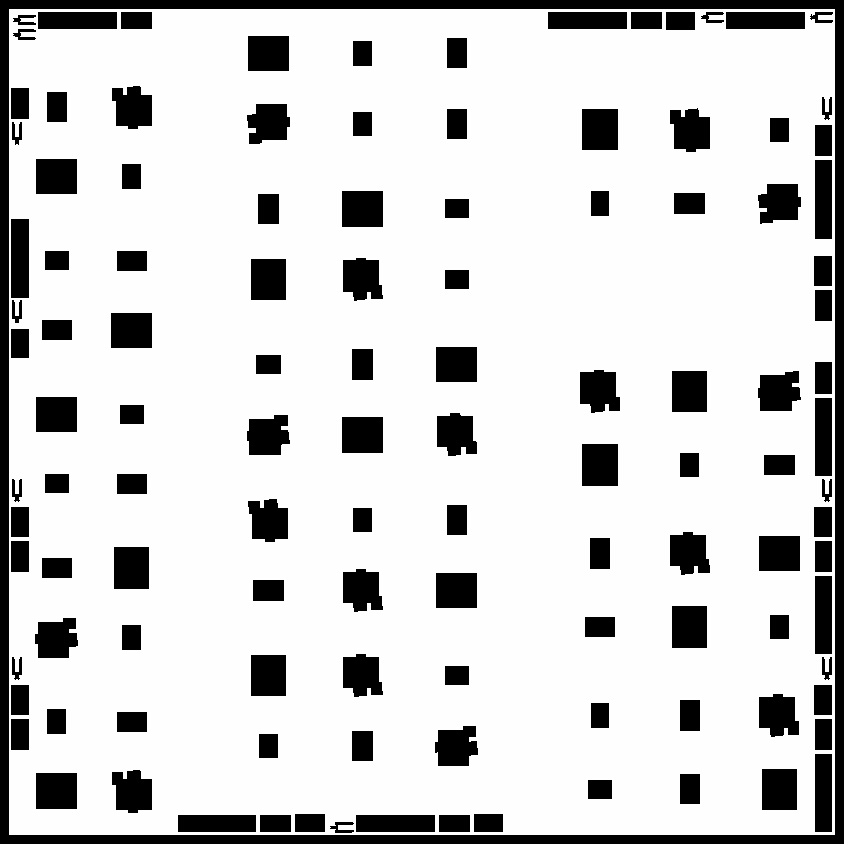
\includegraphics[width=\textwidth]{figures/warehouse_static_01.png}\\[0.4ex]
    {\footnotesize (a) static \texttt{\_01}, distributed}
  \end{minipage}\hfill
  \begin{minipage}[t]{0.32\textwidth}
    \centering
    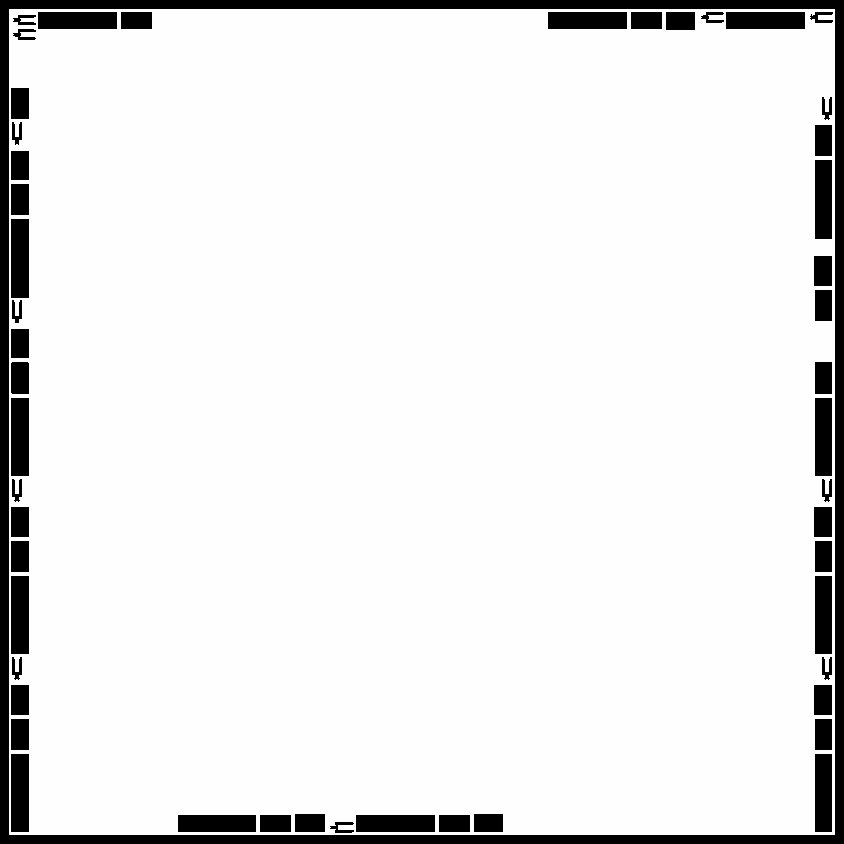
\includegraphics[width=\textwidth]{figures/warehouse_objonwallonly.png}\\[0.4ex]
    {\footnotesize (b) \texttt{objonwallonly}}
  \end{minipage}\hfill
  \begin{minipage}[t]{0.32\textwidth}
    \centering
    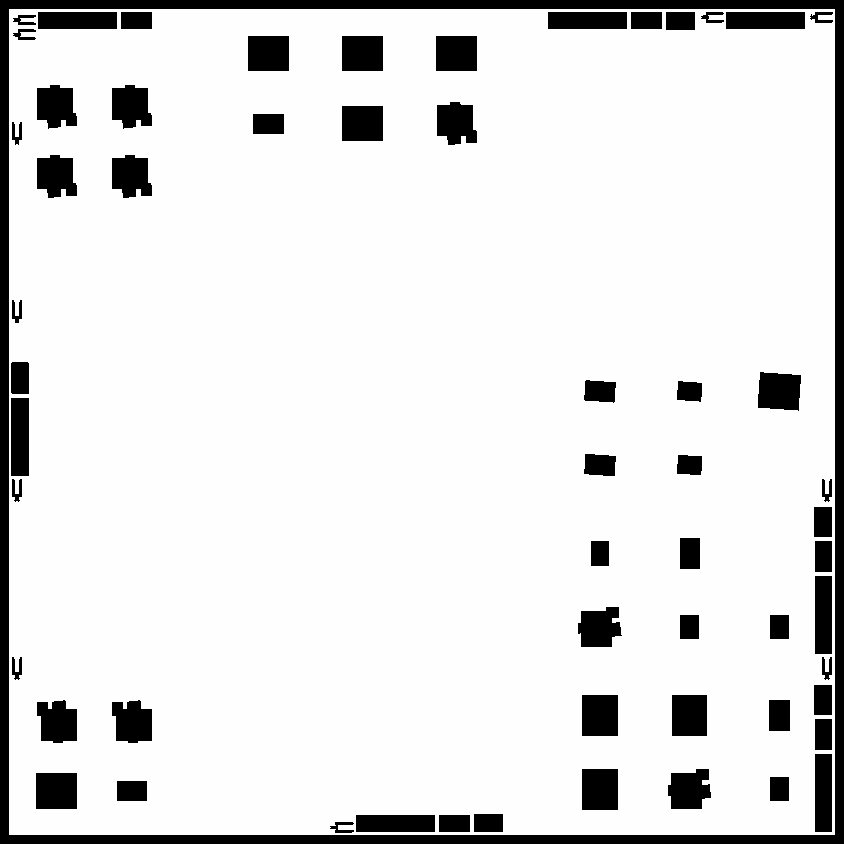
\includegraphics[width=\textwidth]{figures/warehouse_dynamic.png}\\[0.4ex]
    {\footnotesize (c) dynamic}
  \end{minipage}
  \caption[Baked occupancy truth of the three large-warehouse object arrangements, each \SI{42.2}{\metre} square at \SI{0.05}{\metre} per cell with origin $(-21.1,-21.1)$~m.]{Baked occupancy truth of the three large-warehouse object arrangements,
  each \SI{42.2}{\metre} square at \SI{0.05}{\metre} per cell with origin
  $(-21.1,-21.1)$~m. Black is occupied, white is free; there is no unknown space
  because the grids are rasterised from collision geometry rather than observed.
  Occupied cells are \SI{17.79}{\percent} of~(a), \SI{8.74}{\percent} of~(b) and
  \SI{10.98}{\percent} of~(c). Panel~(b) clears the central floor and keeps
  obstacles against the walls, which is the arrangement used by
  \repo{dataset_allsensor_002} and \repo{dataset_allsensor_003}. \emph{No
  occupancy grid is shown per floor treatment, and none exists:} the
  \texttt{bayline} and plain floors differ only in surface material, which carries
  no collision geometry, so their baked grids are identical to the panels above.
  See \cref{fig:floor-treatments}.}
  \label{fig:warehouse-maps}
\end{figure}

The floor treatment is a separate factor and is invisible to occupancy. It is set
by which ground model a world includes; those models share one mesh and differ only
in the visual materials attached to it (\cref{tab:floor-variants}).
\Cref{fig:floor-treatments} renders both recorded conditions at true scale using
\repo{script/render_floor.py}, which drives the 2-D viewer's own floor rasteriser
so that the figure shows what the overlay and the simulated cameras see rather
than a texture file out of context.

\begin{figure}[htbp]
  \centering
  \begin{minipage}[t]{0.33\textwidth}
    \centering
    
\includegraphics[width=\textwidth]{figures/floor_plain.png}\\[0.4ex]
    {\footnotesize (a) plain, \repo{allsensor_000}--\repo{_002}}
  \end{minipage}\hfill
  \begin{minipage}[t]{0.33\textwidth}
    \centering
    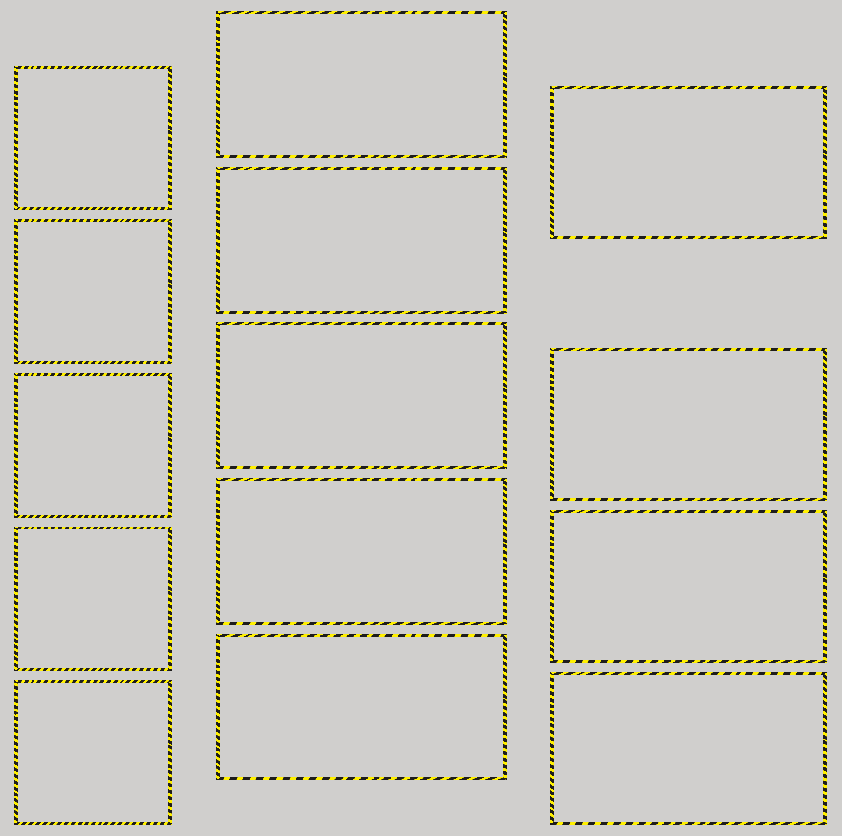
\includegraphics[width=\textwidth]{figures/floor_bayline.png}\\[0.4ex]
    {\footnotesize (b) \texttt{bayline}, \repo{allsensor_003}, \repo{_004}}
  \end{minipage}\hfill
  \begin{minipage}[t]{0.29\textwidth}
    \centering
    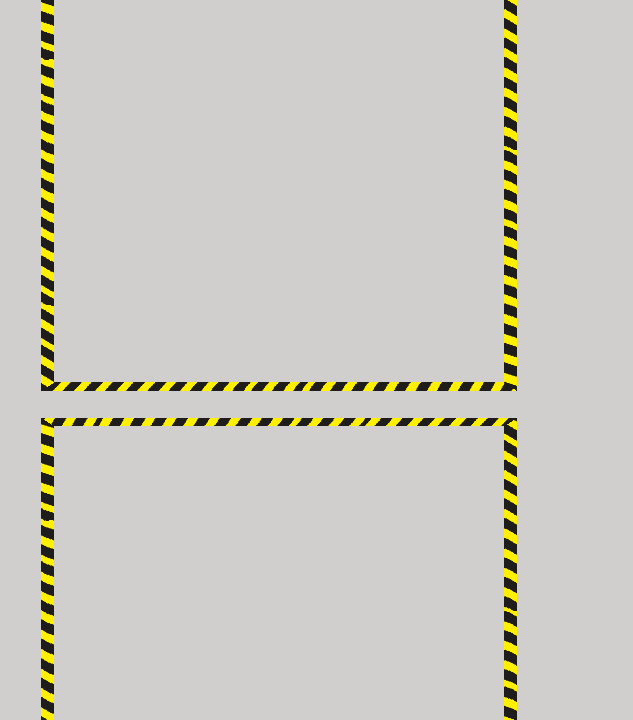
\includegraphics[width=\textwidth]{figures/floor_bayline_detail.png}\\[0.4ex]
    {\footnotesize (c) \SI{12}{\metre} detail of~(b)}
  \end{minipage}
  \caption[The two recorded floor conditions, rendered across the full \SI{42.2}{\metre} floor at \SI{0.05}{\metre} per pixel.]{The two recorded floor conditions, rendered across the full
  \SI{42.2}{\metre} floor at \SI{0.05}{\metre} per pixel. Both share the same flat
  diffuse base, RGB $(0.814,0.811,0.804)$; the only difference between them is the
  112 painted marking faces that \texttt{bayline} adds, forming the hazard-striped
  outlines of fourteen storage bays. Panel~(c) is a \SI{12}{\metre} square detail
  showing the strips at \SI{0.145}{\metre} width. Everything not outlined is
  untextured in both conditions.}
  \label{fig:floor-treatments}
\end{figure}

\begin{table}[htbp]
\centering
\caption[Ground models and the floor conditions they produce.]{Ground models and the floor conditions they produce. The mesh and its
collision geometry are identical in all three, so the floor treatment changes what
a camera sees and nothing a wheel, an occupancy grid or a collision check responds
to. The concrete-grain texture belongs to the stock model only, and no recorded
dataset uses it.}
\label{tab:floor-variants}
\small
\begin{tabularx}{\textwidth}{>{\raggedright\arraybackslash}p{0.29\textwidth}lll>{\raggedright\arraybackslash}X}
\toprule
Ground model & Base & Concrete & Markings & Used by \\
\midrule
\repo{..._GroundB_01} (stock) & texture & yes & 112 faces & no recorded dataset \\
\repo{..._GroundB_01_bayline} & flat diffuse & no & 112 faces &
  \repo{allsensor_003}, \repo{allsensor_004} \\
\repo{..._GroundB_01_plain} & flat diffuse & no & none &
  \repo{allsensor_000}--\repo{_002}, all \texttt{nofloortexture} datasets \\
\bottomrule
\end{tabularx}
\end{table}

\begin{queried}[Naming]
The factor recorded in this project as ``textured versus featureless floor'' is
narrower than the name suggests, and \cref{fig:floor-treatments} is the evidence.
Both conditions rest on the \emph{same flat, untextured diffuse colour}; the stock
concrete-grain texture appears in neither. The entire difference is fourteen
painted bay outlines, \SI{0.145}{\metre} wide, covering a small fraction of a
\SI{1704}{\metre\squared} floor. A robot driving an aisle sees a uniform grey
surface in both conditions for most of its path, crossing a high-contrast strip
only at a bay boundary.

Results comparing the two floors must therefore be read as \emph{bay markings
versus nothing}, not as \emph{realistic floor versus nothing}, and the near-absence
of a visual-odometry improvement between them (\cref{sec:results-proprio}) should
not be generalised to floors carrying genuine surface texture. Testing that would
require a world built on the stock \repo{GroundB_01} model, which no recorded
dataset uses.
\end{queried}

\begin{queried}[Unverified]
The dynamic world's baked grid, \cref{fig:warehouse-maps}(c), contains
\SI{38}{\percent} fewer occupied cells than the distributed static arrangement
in~(a). \repo{bake_map.py} rasterises every \texttt{<include>} in the
world file at its authored pose, so kinematically driven props should appear at
their initial positions, but this has not been confirmed for the dynamic family.
Until it is, panel~(c) must not be used as occupancy truth for scoring a
reconstructed map of a dynamic scene: the deficit may be a genuine difference in
static stocking, or it may be props missing from the bake, and those two
possibilities imply opposite corrections. The estimator results in
\cref{sec:results-proprio} are unaffected, as they use the arrangements in
panels~(a) and~(b) only.
\end{queried}

Each recorded dataset is the combination of three things that vary independently
and are easy to confuse when read off three separate artifacts: the floor
treatment, the object arrangement, and the route the robot actually drove.
\Cref{fig:dataset-scenes} draws all three together for every dataset, and
\cref{tab:dataset-scenes} gives the numbers behind the pictures. Both are produced
by \repo{script/render_dataset_scene.py}, which resolves each dataset's world from
its own run manifest rather than from its name---necessary because
\repo{dataset_static_nofloortexture_001} sits in the \texttt{\_01} arrangement
while \repo{_000} and \repo{_002} sit in the canonical one, and all three carry
\texttt{nofloortexture} in the name.

\begin{figure}[p]
  \centering
  \begin{minipage}[t]{0.235\textwidth}
    \centering
    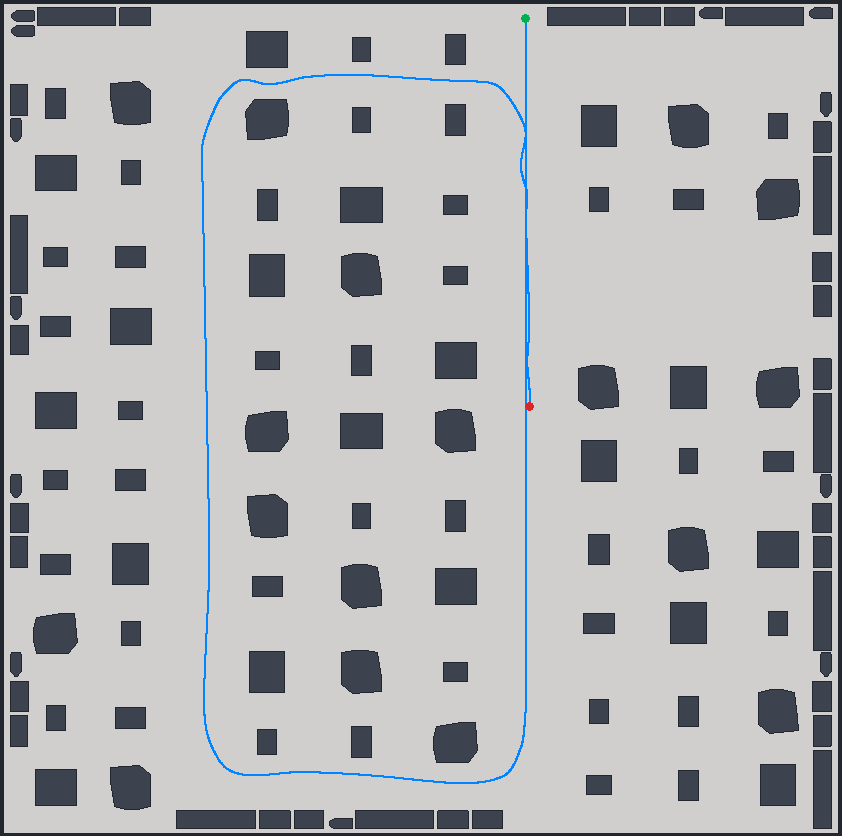
\includegraphics[width=\textwidth]{figures/scene_allsensor_000.png}\\[0.3ex]
    {\scriptsize \repo{allsensor_000}}
  \end{minipage}\hfill
  \begin{minipage}[t]{0.235\textwidth}
    \centering
    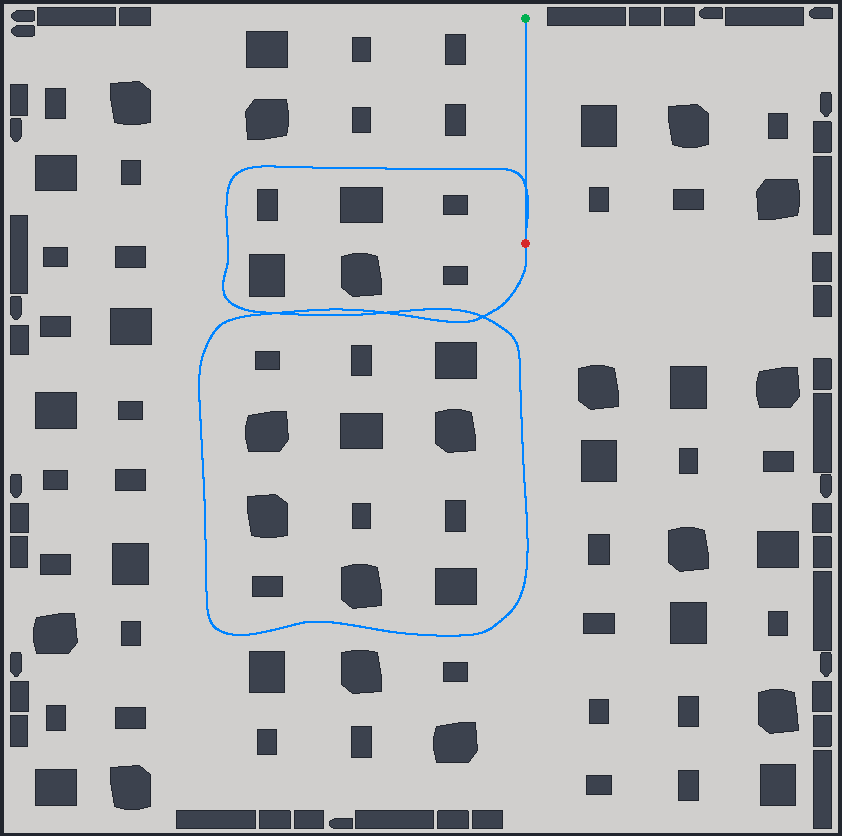
\includegraphics[width=\textwidth]{figures/scene_allsensor_001.png}\\[0.3ex]
    {\scriptsize \repo{allsensor_001}}
  \end{minipage}\hfill
  \begin{minipage}[t]{0.235\textwidth}
    \centering
    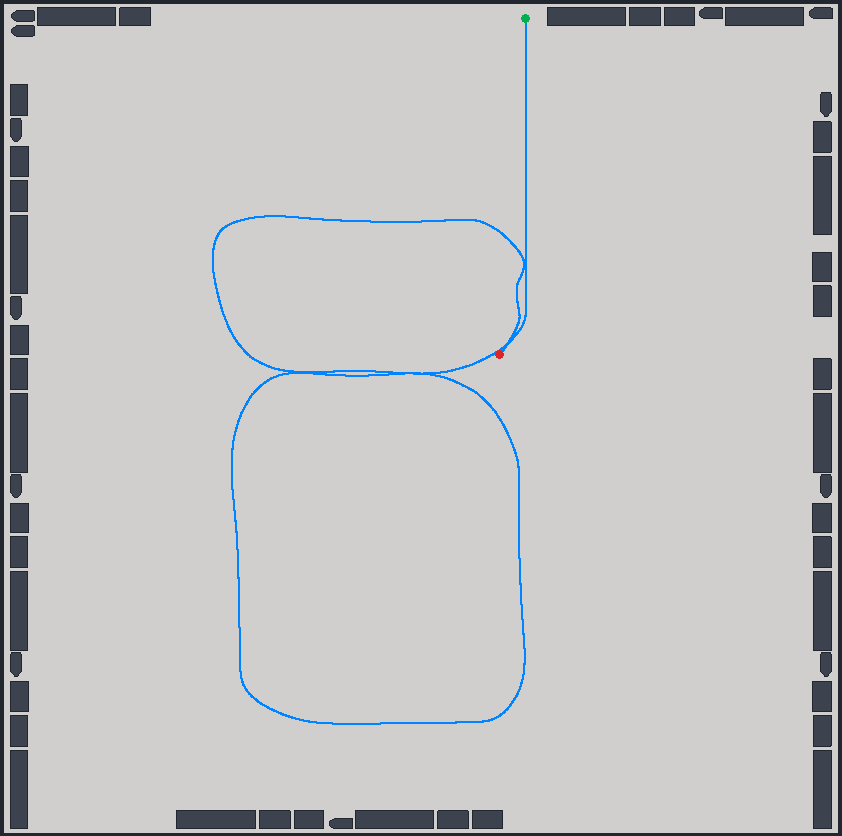
\includegraphics[width=\textwidth]{figures/scene_allsensor_002.png}\\[0.3ex]
    {\scriptsize \repo{allsensor_002}}
  \end{minipage}\hfill
  \begin{minipage}[t]{0.235\textwidth}
    \centering
    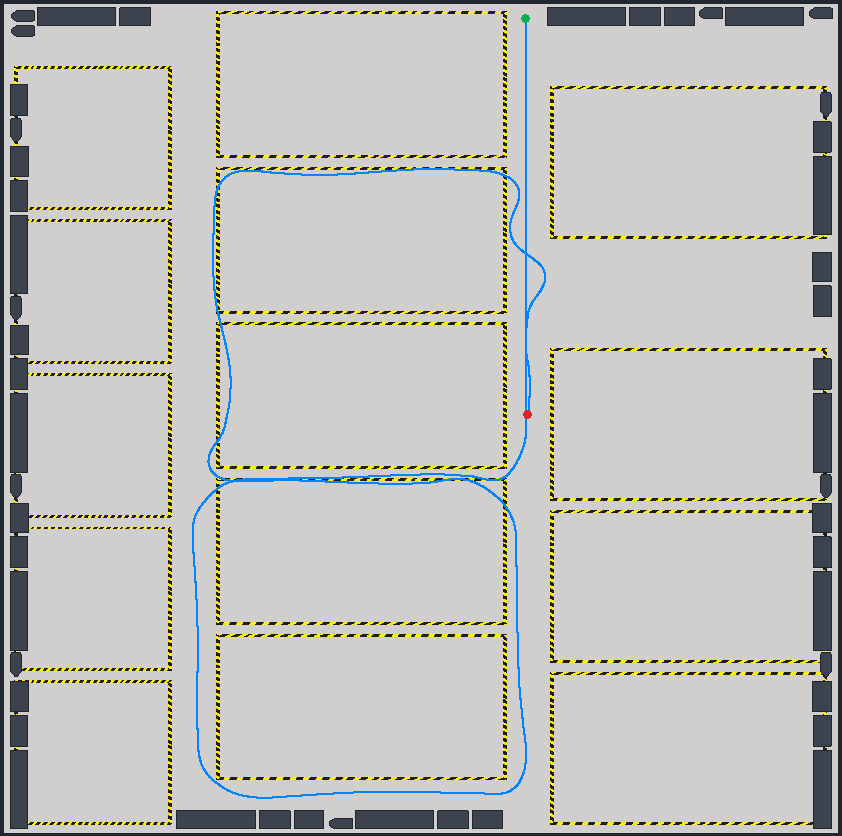
\includegraphics[width=\textwidth]{figures/scene_allsensor_003.png}\\[0.3ex]
    {\scriptsize \repo{allsensor_003}}
  \end{minipage}

  \vspace{1.2ex}
  \begin{minipage}[t]{0.235\textwidth}
    \centering
    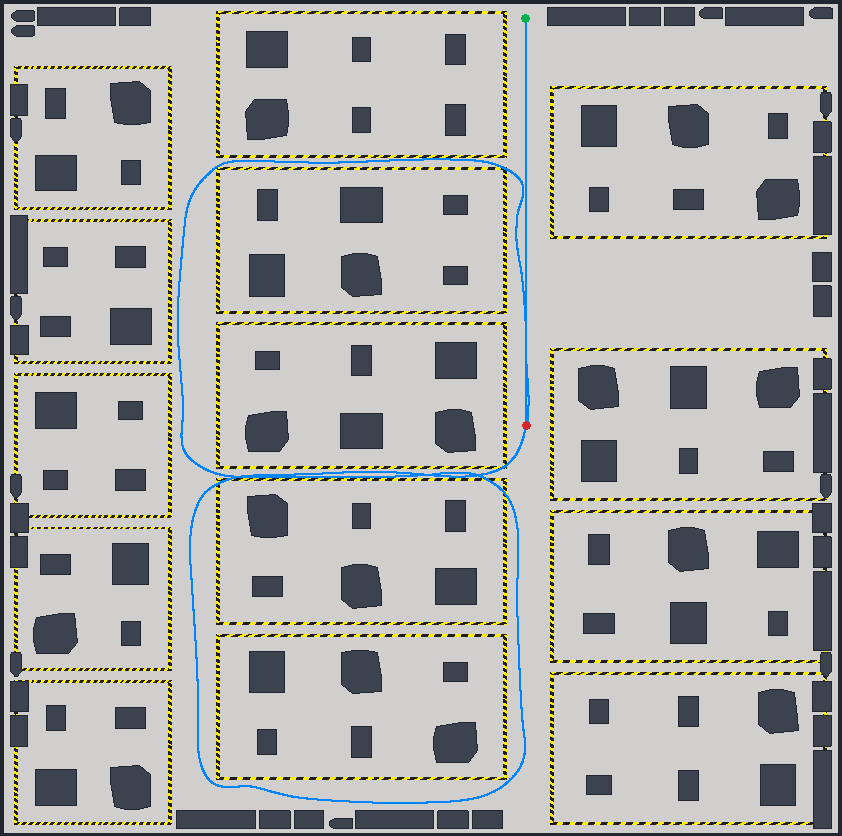
\includegraphics[width=\textwidth]{figures/scene_allsensor_004.png}\\[0.3ex]
    {\scriptsize \repo{allsensor_004}}
  \end{minipage}\hfill
  \begin{minipage}[t]{0.235\textwidth}
    \centering
    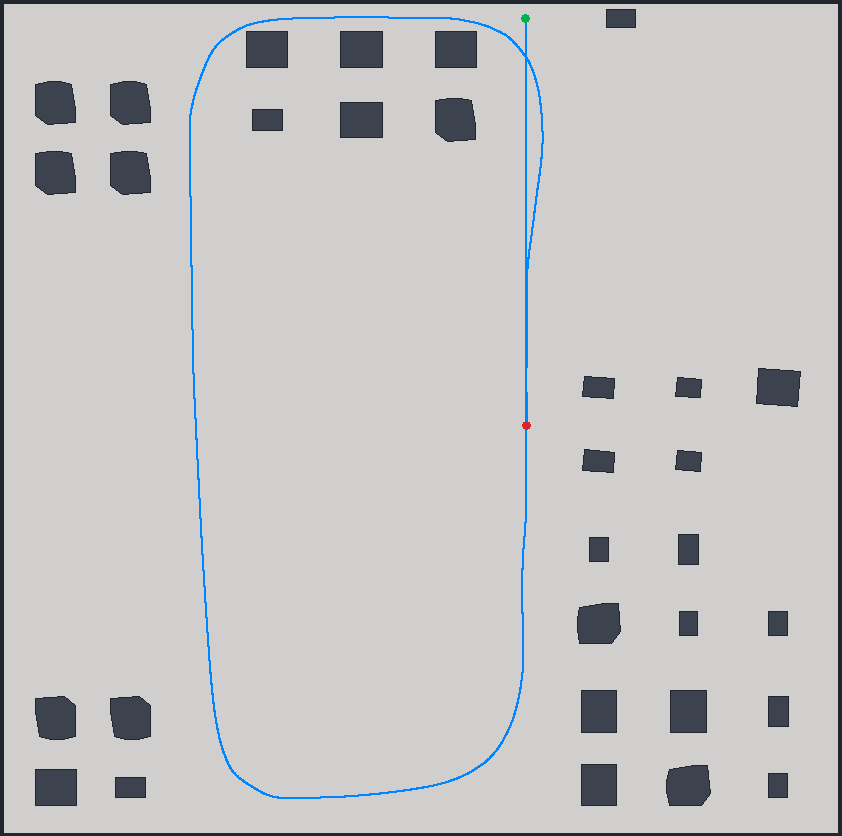
\includegraphics[width=\textwidth]{figures/scene_static_nofloortexture_000.png}\\[0.3ex]
    {\scriptsize \repo{static_000}\flag{*}}
  \end{minipage}\hfill
  \begin{minipage}[t]{0.235\textwidth}
    \centering
    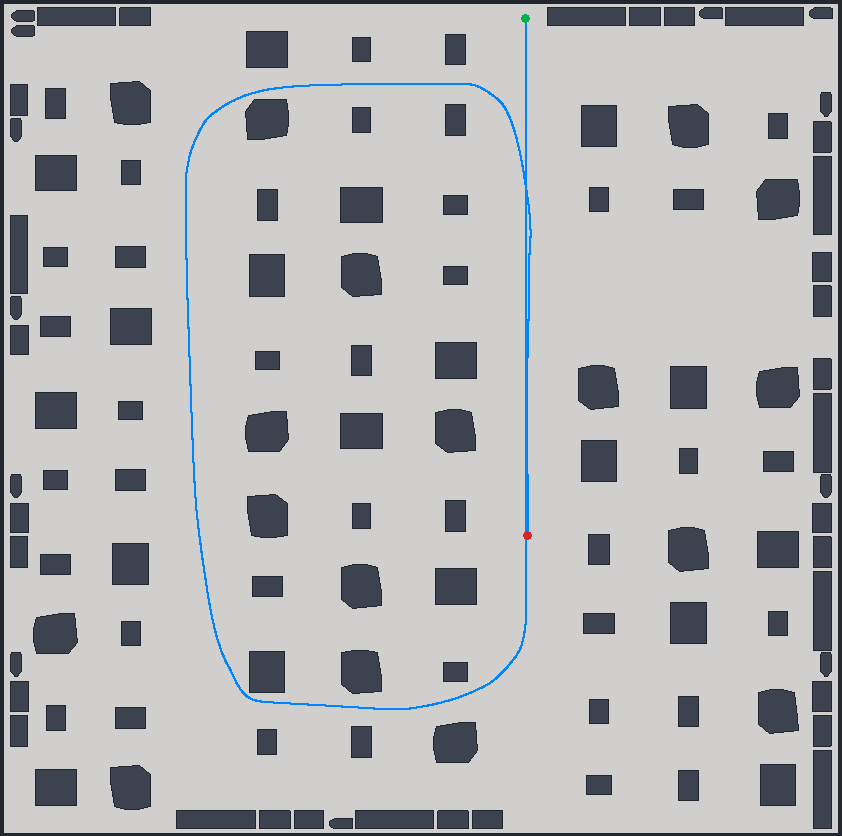
\includegraphics[width=\textwidth]{figures/scene_static_nofloortexture_001.png}\\[0.3ex]
    {\scriptsize \repo{static_001}}
  \end{minipage}\hfill
  \begin{minipage}[t]{0.235\textwidth}
    \centering
    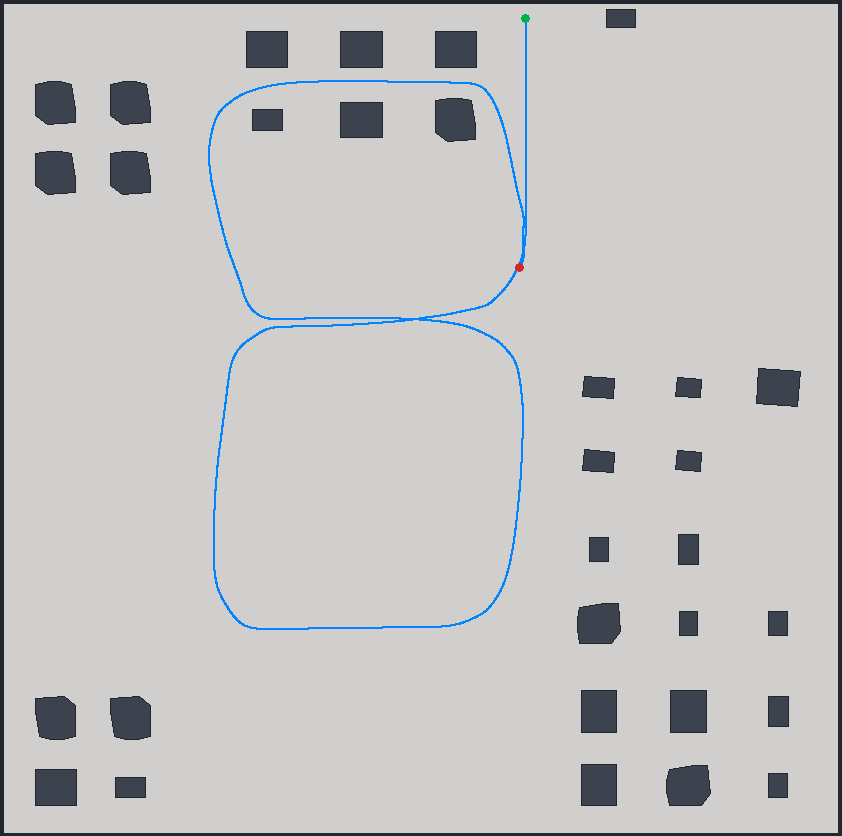
\includegraphics[width=\textwidth]{figures/scene_static_nofloortexture_002.png}\\[0.3ex]
    {\scriptsize \repo{static_002}\flag{*}}
  \end{minipage}

  \vspace{1.2ex}
  \begin{minipage}[t]{0.235\textwidth}
    \centering
    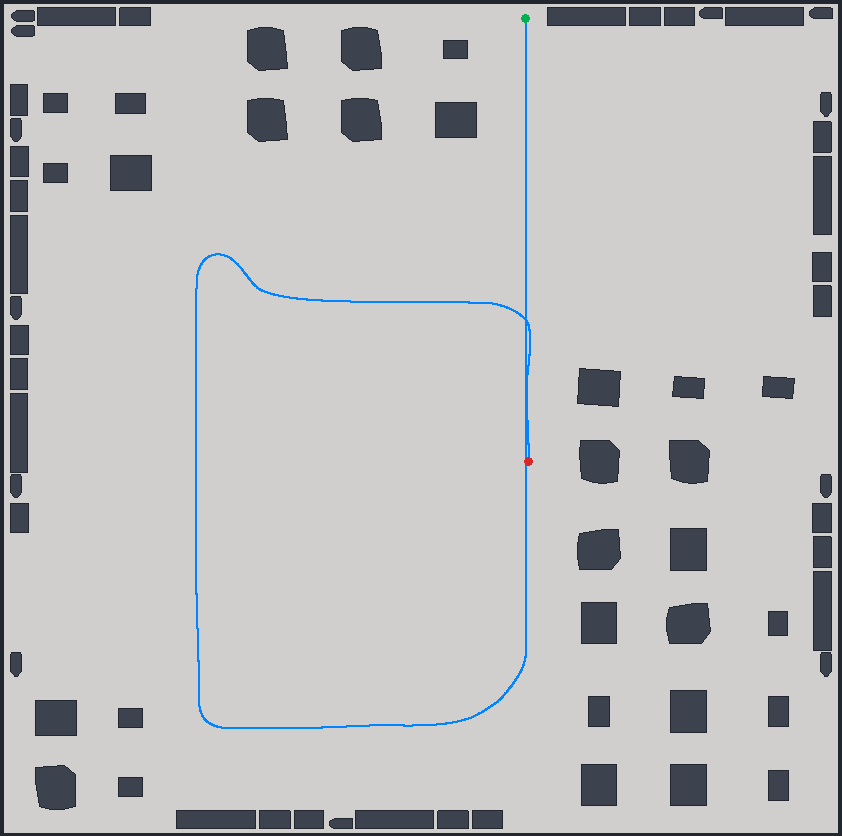
\includegraphics[width=\textwidth]{figures/scene_dynamic_nofloortexture_00_000.png}\\[0.3ex]
    {\scriptsize \repo{dynamic_00_000}}
  \end{minipage}\hfill
  \begin{minipage}[t]{0.235\textwidth}
    \centering
    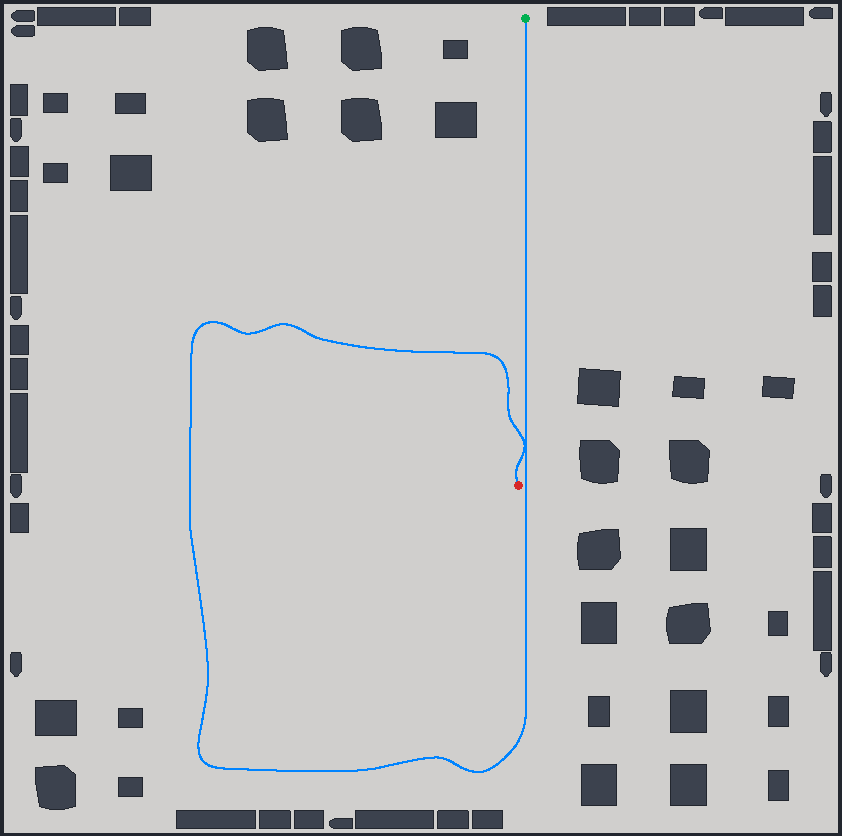
\includegraphics[width=\textwidth]{figures/scene_dynamic_nofloortexture_00_001.png}\\[0.3ex]
    {\scriptsize \repo{dynamic_00_001}}
  \end{minipage}\hfill
  \begin{minipage}[t]{0.235\textwidth}
    \centering
    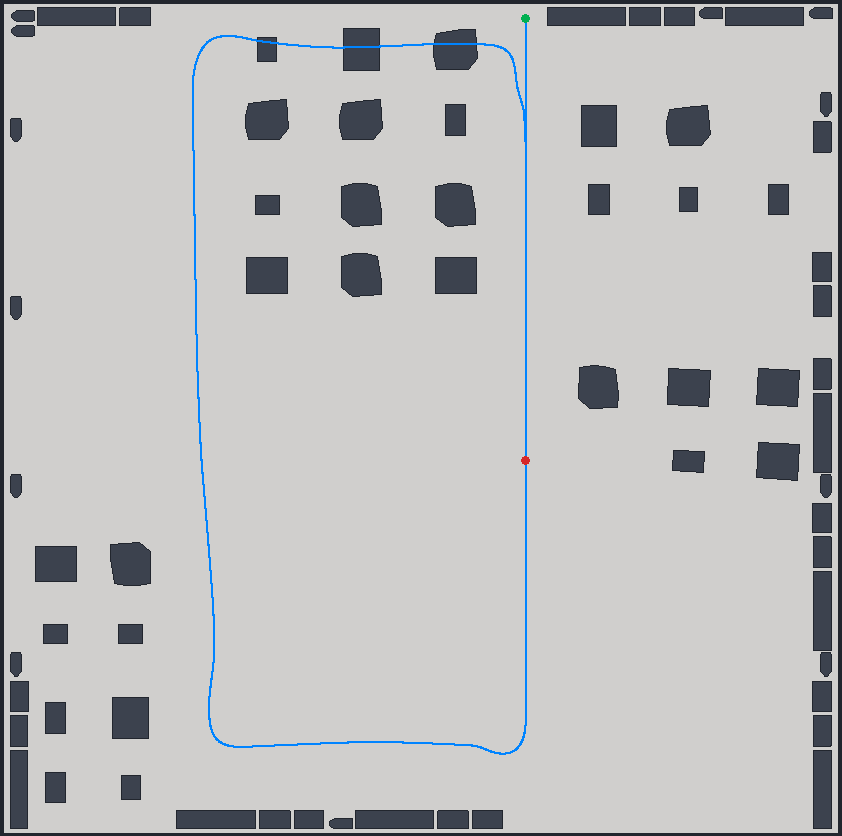
\includegraphics[width=\textwidth]{figures/scene_dynamic_nofloortexture_01_000.png}\\[0.3ex]
    {\scriptsize \repo{dynamic_01_000}}
  \end{minipage}\hfill
  \begin{minipage}[t]{0.235\textwidth}
    \centering
    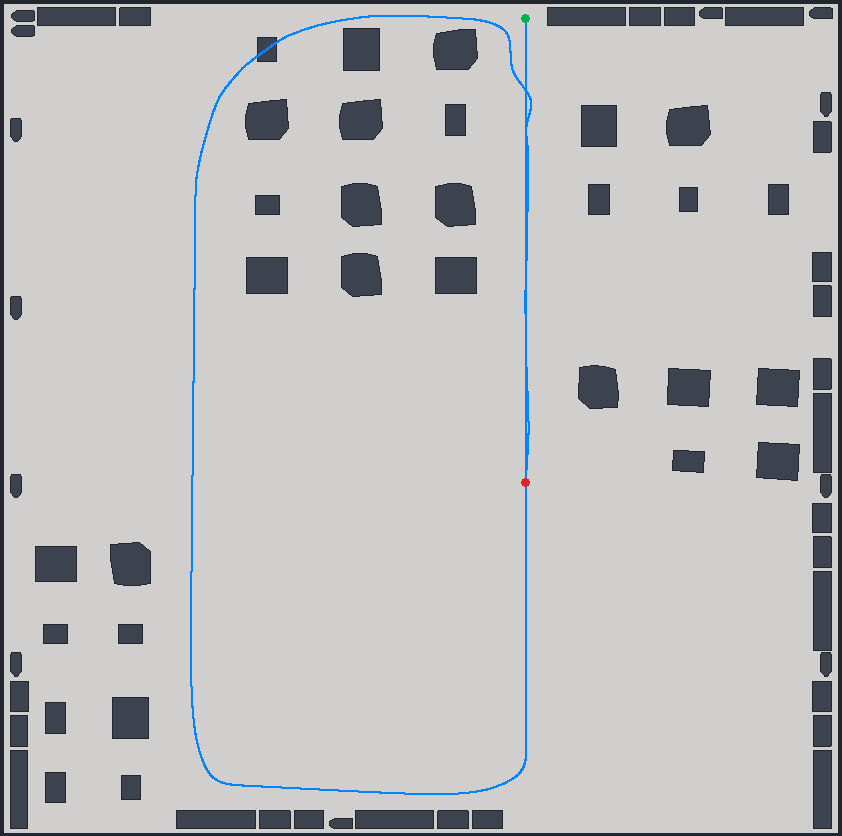
\includegraphics[width=\textwidth]{figures/scene_dynamic_nofloortexture_02_000.png}\\[0.3ex]
    {\scriptsize \repo{dynamic_02_000}}
  \end{minipage}
  \caption[Every simulation dataset as a scene: floor treatment, object layout and ground-truth route in one view.]{Every simulation dataset as a scene: floor treatment, object layout and
  ground-truth route in one view. Grey is open floor; dark polygons are obstacle
  footprints, taken as convex hulls of each collision mesh sliced at robot height,
  the same geometry the occupancy bake uses. Yellow hazard striping is the painted
  bay outline of the \texttt{bayline} floor and is absent on plain floors. The blue
  trace is the recorded \repo{/ground_truth/odometry} route, green marking its
  start and red its end. Moving props are drawn at their authored pose, which is
  where the world file places them at $t=0$; this is a layout figure and does not
  show where a prop was at any instant during a dynamic recording. \flag{*}~marks a
  dataset whose recorded world no longer exists and whose objects were
  reconstructed---see the note below \cref{tab:dataset-scenes}.}
  \label{fig:dataset-scenes}
\end{figure}

\begin{table}[htbp]
\centering
\caption[What each dataset contains.]{What each dataset contains. ``Objects'' counts obstacle instances whose
collision geometry intersects the robot-height band, excluding the wall ring.
``Route'' is the ground-truth path length and ``sim span'' its duration in
simulated time. The world column drops the floor suffix, which is given separately,
so two rows sharing a world arrangement but differing in floor are visible as such.}
\label{tab:dataset-scenes}
\footnotesize
\setlength{\tabcolsep}{3pt}
%% Generated by script/render_dataset_scene.py -- do not edit.
\begin{tabularx}{\textwidth}{>{\raggedright\arraybackslash}Xllrrrr}
\toprule
Dataset & World & Floor & Objects & Route & Sim span & Truth \\
 & arrangement & & & [\si{\metre}] & [\si{\second}] & samples \\
\midrule
\repo{dataset_allsensor_000} & \texttt{static\_01} & plain & 117 & 117.0 & 87.1 & 4354 \\
\repo{dataset_allsensor_001} & \texttt{static\_01} & plain & 117 & 113.1 & 81.8 & 4091 \\
\repo{dataset_allsensor_002} & \texttt{static\_objonwallonly} & plain & 49 & 115.2 & 86.7 & 4338 \\
\repo{dataset_allsensor_003} & \texttt{static\_objonwallonly} & bayline & 49 & 140.6 & 102.4 & 5119 \\
\repo{dataset_allsensor_004} & \texttt{static\_01} & bayline & 117 & 142.3 & 100.5 & 5026 \\
\repo{dataset_dynamic_nofloortexture_00_000} & \texttt{dynamic\_00} & plain & 69 & 97.1 & 77.4 & 3873 \\
\repo{dataset_dynamic_nofloortexture_00_001} & \texttt{dynamic\_00} & plain & 69 & 97.3 & 74.2 & 3710 \\
\repo{dataset_dynamic_nofloortexture_01_000} & \texttt{dynamic\_01} & plain & 68 & 122.8 & 84.6 & 4230 \\
\repo{dataset_dynamic_nofloortexture_02_000} & \texttt{dynamic\_02} & plain & 68 & 126.6 & 89.5 & 4475 \\
\repo{dataset_static_nofloortexture_000}\flag{*} & \texttt{static} & plain & 31 & 122.9 & 86.7 & 4334 \\
\repo{dataset_static_nofloortexture_001} & \texttt{static\_01} & plain & 117 & 113.1 & 82.0 & 4100 \\
\repo{dataset_static_nofloortexture_002}\flag{*} & \texttt{static} & plain & 31 & 114.7 & 89.5 & 4475 \\
\bottomrule
\end{tabularx}

\end{table}

\begin{queried}[Missing world]
\repo{dataset_static_nofloortexture_000} and \repo{_002} name
\repo{worlds/small_warehouse_static/small_warehouse_static_nofloortexture.world}
in their run manifests, and \flag{that file no longer exists in the repository}.
Both datasets contribute to the relogged campaign of \cref{sec:results-validity},
so their scenes could not be drawn from the recorded world and their conditions
cannot be re-inspected directly.

The panels marked \flag{*} are reconstructions. They are exact for geometry rather
than approximate, because \repo{script/make_plain_floor.py} produces a floor
variant by swapping only the ground model's \texttt{<include>} URI and leaves every
object untouched: the missing world therefore differed from the surviving
\repo{small_warehouse_static.world} in its floor alone, and that floor is
recoverable from the suffix. It remains a reconstruction and not the recorded file,
and the two datasets should be re-recorded, or the world restored from history,
before either is used for anything the floor or the object layout bears on.
\end{queried}

The available controlled factors are summarised in \cref{tab:controlled-factors}.

\begin{table}[htbp]
\centering
\caption[Controlled experimental factors available in the simulation environment, with the levels realised at the reporting cutoff.]{Controlled experimental factors available in the simulation environment,
with the levels realised at the reporting cutoff. A factor is listed as exercised
only where a recorded dataset exists for more than one of its levels.}
\label{tab:controlled-factors}
\small
\begin{tabularx}{\textwidth}{>{\raggedright\arraybackslash}p{0.21\textwidth}>{\raggedright\arraybackslash}p{0.30\textwidth}>{\raggedright\arraybackslash}X}
\toprule
Factor & Levels & Status at cutoff \\
\midrule
Scene dynamics & static props; scripted dynamic props & exercised \\
Floor markings & bay outlines present (\texttt{bayline});
  absent (plain) & exercised; no dataset carries surface texture \\
Prop or route arrangement & canonical; \texttt{\_00}; \texttt{\_01};
  \texttt{\_02} & exercised \\
Stocking level & partial; fully stocked static & fully stocked recorded \\
Object placement & distributed; restricted to the wall region & exercised, three
  bags to one \\
Domain & simulation; real robot & exercised, no real ground truth \\
World scale & tiny \repo{small_warehouse}; large rescaled families & distinct
  environments, never pooled \\
\bottomrule
\end{tabularx}
\end{table}

The plain floor removes the painted bay outlines; neither recorded condition
carries the stock concrete texture. Collision geometry and occupancy truth are
preserved in both (\cref{tab:floor-variants}). Dynamic props follow
deterministic routes through a kinematic Gazebo plugin. This preserves repeatable
motion and acceptable real-time factor, but it does not reproduce physical
collision response if the robot overlaps a moving prop.

World identity is recorded by exact \texttt{.world} path. ROS launches require
\repo{colcon build --symlink-install}; a plain build can leave an obsolete copied
world in \repo{install/}. When object motion is required by the 2-D viewer, model
poses must also be bridged from the simulator.


\subsection{Dataset registry}
\label{sec:dataset-registry}
% Verbatim from minor_report/chapters/chapter_3_methodology.tex lines 910-1043 (retired report),
% headings demoted by 0 level(s). Do not edit here; edit the source of the numbers.

Datasets are held in two places and the registry must cover both: the workspace
tree \repo{dataset/} and a removable drive mounted at
\repo{/media/ambushee/32E4AAB1E4AA772F/}, whose simulation bags sit under
\repo{dataset/} and whose real-robot recordings sit at its root.
\Cref{tab:dataset-registry} lists all eighteen recordings across both locations.
Six exist in one place only on the drive, seven in the workspace only, and three
are held in both.

\begin{sidewaystable}[p]
\centering
\caption[Complete dataset registry at the reporting cutoff, across both storage locations.]{Complete dataset registry at the reporting cutoff, across both storage
locations. The \texttt{bayline} families carry a textured floor; every other
simulation entry is featureless. ``WS'' is the workspace tree \repo{dataset/} and ``FD'' the removable
drive; a size is given where that location holds a copy. ``Prop.'' marks the
proprioceptive group (\repo{/model/ackermann_robot_001/joint_state} and
\repo{/model/ackermann_robot_001/odometry}); ``IMU'' counts inertial messages,
on \repo{/imu} for simulation and \repo{/hwt101ct_yaw_publisher} for the real
rig. Durations are rosbag wall-clock recording durations: the simulator ran below
real time, so a bag's sim-time span is shorter than the figure shown. Integrity
was checked by opening each SQLite store and counting rows against the count its
\repo{metadata.yaml} declares, not by trusting the metadata.}
\label{tab:dataset-registry}
\scriptsize
\setlength{\tabcolsep}{4pt}
\begin{tabular}{llrrrrcccl}
\toprule
Dataset & Family & WS & FD & Dur.\ (s) & Messages & \texttt{/clock} & Truth &
  Prop. & Integrity \\
 & & (MB) & (MB) & & & & & & \\
\midrule
\repo{dataset_allsensor_000} & static \texttt{\_01} & 689 & -- & 129.3 & 211\,811 &
  \checkmark & \checkmark & \checkmark & ok \\
\repo{dataset_allsensor_001} & static \texttt{\_01} & 674 & -- & 126.2 & 198\,873 &
  \checkmark & \checkmark & \checkmark & ok \\
\repo{dataset_allsensor_002} & static, wall only & 750 & -- & 105.5 & 215\,528 &
  \checkmark & \checkmark & \checkmark & ok \\
\repo{dataset_allsensor_003} & bayline, wall only & 1056 & -- & 141.2 & 255\,699 &
  \checkmark & \checkmark & \checkmark & ok \\
\repo{dataset_allsensor_004} & bayline, distributed & 1311 & -- & 168.6 & 253\,942 &
  \checkmark & \checkmark & \checkmark & ok \\
\midrule
\repo{dataset_static_nofloortexture_000} & static & -- & 592 & 101.5 & 118\,597 &
  \checkmark & \checkmark & -- & ok \\
\repo{dataset_static_nofloortexture_001} & static & 617 & 1 & 92.0 & 113\,332 &
  \checkmark & \checkmark & -- & \flag{FD stub, WS ok} \\
\repo{dataset_static_nofloortexture_002} & static & -- & 688 & 103.3 & 122\,386 &
  \checkmark & \checkmark & -- & ok \\
\repo{dataset_static_nofloortexture_objonwallonly} & static, wall only & 648 & -- &
  110.5 & 114\,523 & \checkmark & \checkmark & -- & ok \\
\midrule
\repo{dataset_dynamic_nofloortexture_00_000} & dynamic \texttt{\_00} & -- & 653 &
  100.3 & 111\,988 & \checkmark & \checkmark & -- & ok \\
\repo{dataset_dynamic_nofloortexture_00_001} & dynamic \texttt{\_00} & -- & 778 &
  167.7 & 114\,169 & \checkmark & \checkmark & -- & ok \\
\repo{dataset_dynamic_nofloortexture_01_000} & dynamic \texttt{\_01} & 713 & 710 &
  165.4 & 126\,790 & \checkmark & \checkmark & -- & \flag{FD malformed, WS ok} \\
\repo{dataset_dynamic_nofloortexture_02_000} & dynamic \texttt{\_02} & -- & 758 &
  172.1 & 134\,995 & \checkmark & \checkmark & -- & ok \\
\midrule
\repo{dataset_map_01} & mapping, large & 818 & -- & 193.5 & 152\,291 & \checkmark &
  \checkmark & -- & ok \\
\repo{dataset_map_tiny} & mapping, tiny world & 726 & -- & 63.3 & 82\,555 &
  \checkmark & \checkmark & -- & ok \\
\midrule
\repo{dataset_real_000} & real rig & 2964 & 2964 & 116.6 & 36\,166 & -- & -- & -- &
  ok, 23\,257 IMU \\
\repo{dataset_real_001} & real rig & -- & 2099 & 85.5 & 9\,629 & -- & -- & -- &
  \flag{0 IMU messages} \\
\repo{dataset_real_002} & real rig & -- & 2869 & 113.5 & 12\,682 & -- & -- & -- &
  \flag{0 IMU messages} \\
\bottomrule
\end{tabular}
\end{sidewaystable}

The seven featureless-floor simulation bags of the relogged campaign
(\cref{sec:results-validity}) are the static and dynamic families listed above;
five were read from the drive and two from the workspace, for the reason recorded
next.

\begin{queried}[Data integrity]
Two drive copies are unreadable while presenting a complete, plausible
\repo{metadata.yaml}. \repo{dataset_static_nofloortexture_001} is a
\SI{524288}{\byte} stub whose metadata nevertheless declares 113\,332 messages,
and \repo{dataset_dynamic_nofloortexture_01_000} is \SI{710}{\mega\byte}---within
\SI{0.4}{\percent} of its workspace counterpart---with a valid SQLite header but a
store that reports \emph{database disk image is malformed} on any query. Both have
intact workspace copies, which is why those two datasets were read from the
workspace in the relogged campaign.

The general lesson is recorded as a control rather than an incident:
\repo{metadata.yaml} is written when recording begins and does not describe what
survived, so message counts, durations and topic lists copied from it are not
evidence that a bag is intact. Storage health must be established by opening the
SQLite store and counting rows, which is now part of the pre-experiment inspection
in \cref{sec:collection-validity}.
\end{queried}

\begin{queried}[Scope limit]
Only the five \repo{dataset_allsensor} bags carry wheel encoders and wheel
odometry; the other thirteen recordings omit those topics entirely. The
proprioceptive baseline of \cref{sec:results-proprio} therefore cannot be computed
for any dynamic condition, for the mapping bags, or for the real rig, and the
comparison between proprioception and visual odometry exists only in
\emph{static, featureless-floor} scenes---the conditions least favourable to
vision and most favourable to dead reckoning. Extending it requires re-recording
with the two topics bridged, not new analysis.
\end{queried}

\begin{queried}[Excluded]
\repo{dataset_real_001} and \repo{dataset_real_002} are excluded because their
inertial topic \repo{/hwt101ct_yaw_publisher} contains \emph{zero} messages, so
neither supports stereo-inertial operation at all. Their image streams are intact
(2\,562 and 3\,405 pairs), so they remain usable for detector or image-only work.
\repo{dataset_real_000} is the only real recording with inertial data, at 23\,257
messages.
\end{queried}

Historical output folders do not prove that their raw bags remain available or
valid. Conversely, a dataset is not marked broken merely because its only copy
lives on the removable drive rather than in the repository; six of the fifteen
recordings are drive-only and are sound.

Before a new experiment, the bag's absolute path, topics, duration, message
counts, and storage health are inspected. Each paired comparison uses the same
recording, and estimators run separately to avoid resource-contention effects.
Environment, trajectory, calibration, replay rate, image transport,
initialization treatment, and revision are controlled. A run is excluded if
input overlap, initialization, processed sample count, or sensor delivery differs
materially from its paired condition.

Recorded simulation bags used by RTAB-Map contain \texttt{/clock}. They are
played without rosbag's additional \texttt{--clock} option because competing
clock sources cause TF time jumps. This choice is made after inspecting each bag,
not applied as a universal command rule.


\section{Real Platform}
\label{sec:real-platform}

\subsection{AMR mobile robot testbed}

The system is installed and tested on a Gensurv Robotics mobile-robot base
designed to reproduce the behaviour of an industrial warehouse AMR
(\cref{fig:amr-dimensions,fig:amr-hardware}). Its maximum speed is set to
\SI{1.5}{\metre\per\second}, the limit of the SLAM stability tests. The
drivetrain is a rear brushless motor (Flipsky 6384) through a BLDC drive with
a Dynamixel RX-64 steering servo, a GigaDevice GD32407V microcontroller on a CAN
link to the NRU-51V, an LM2596 regulator from a lithium-polymer pack, and a
Wi-Fi router for tele-operation from a smartphone.
\flag{The faculty template describes the base as a differential-drive robot;
the hardware diagram (a single traction motor with a steering servo) and the
simulated model of \cref{fig:ackermann-robot} are Ackermann. The description
here follows the hardware and should be confirmed by the author.}

\begin{figure}[htbp]
  \centering
  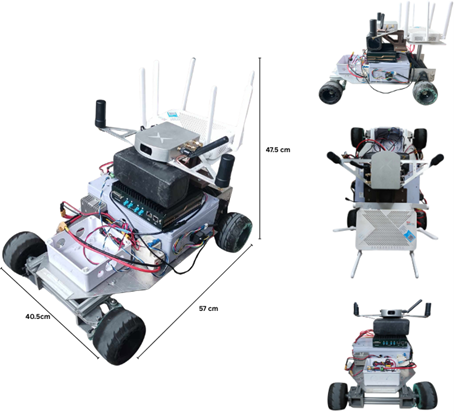
\includegraphics[width=0.75\textwidth]{figures/template/amr_dimensions.png}
  \caption{Dimensions of the mock AMR used to test the navigation system:
  \SI{57}{\centi\metre} long, \SI{40.5}{\centi\metre} wide and
  \SI{47.5}{\centi\metre} high to the top of the sensor mast.}
  \label{fig:amr-dimensions}
\end{figure}

\begin{figure}[htbp]
  \centering
  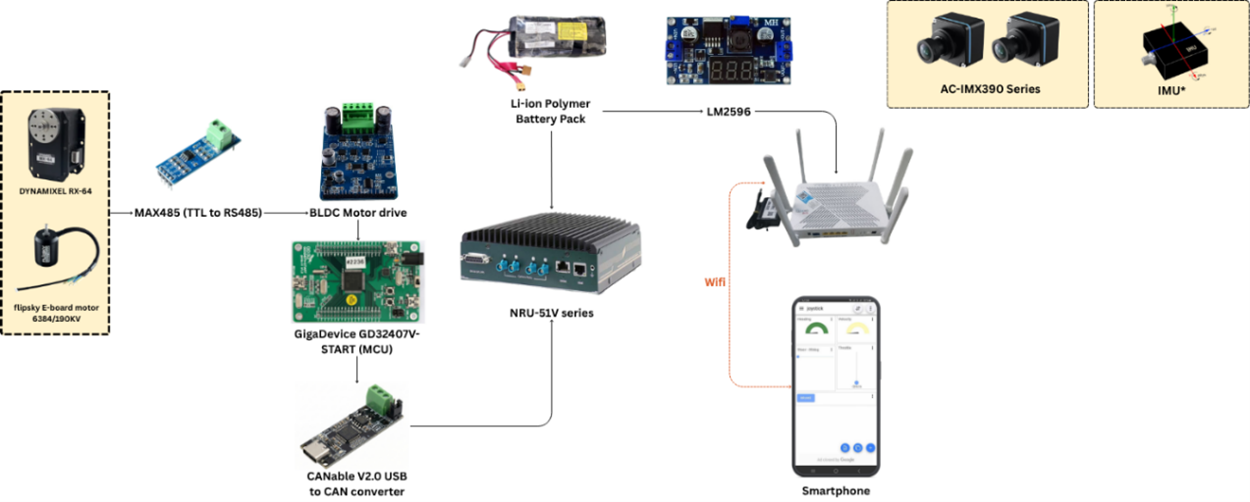
\includegraphics[width=\textwidth]{figures/template/amr_hardware.png}
  \caption[Hardware components of the mock AMR: steering servo and traction motor, BLDC drive and microcontroller on CAN, the NRU-51V computer, power supply, the AC-IMX390 stereo pair and IMU, and the Wi-Fi link to the smartphone joystick.]{Hardware components of the mock AMR: steering servo and traction
  motor, BLDC drive and microcontroller on CAN, the NRU-51V computer, power
  supply, the AC-IMX390 stereo pair and IMU, and the Wi-Fi link to the
  smartphone joystick.}
  \label{fig:amr-hardware}
\end{figure}

\subsection{Sensors and computing unit}

\textbf{Wide-angle stereo cameras (AC-IMX390-H190).} Two AC-IMX390-H190
modules form the stereo pair (\cref{fig:camera-dimensions});
\cref{tab:camera-spec} lists the specification.

\begin{figure}[htbp]
  \centering
  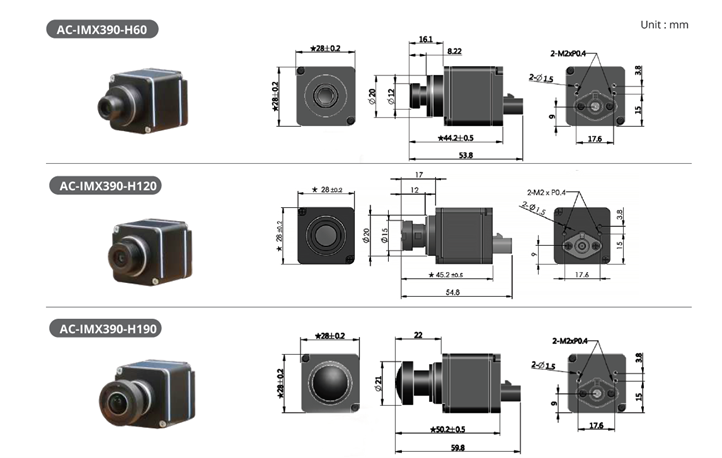
\includegraphics[width=0.9\textwidth]{figures/template/camera_dimensions.png}
  \caption{Dimensions of the AC-IMX390 camera family in millimetres; the
  H190 variant at the bottom is the one used.}
  \label{fig:camera-dimensions}
\end{figure}

\begin{table}[htbp]
\centering
\caption{Specification of the AC-IMX390-H190 camera.}
\label{tab:camera-spec}
\small
\begin{tabularx}{\textwidth}{>{\raggedright\arraybackslash}p{0.30\textwidth}>{\raggedright\arraybackslash}X}
\toprule
Item & Detail \\
\midrule
Sensor and ISP & Sony IMX390 CMOS sensor with GEO Semiconductor GW5200 ISP \\
Resolution and frame rate & $1920\times1080$ (2\,MP) at \SI{30}{fps} \\
Horizontal field of view & \SI{186}{\degree} \\
Video output & uncompressed YUV422 (UYVY) \\
Dynamic range & \SI{120}{\decibel} high dynamic range (HDR) \\
Special features & LED flicker mitigation (LFM), 5-axis active alignment \\
Environmental rating & IP67 and IP69K (lens side) \\
Operating temperature & \SIrange{-40}{85}{\celsius} \\
Connector & male FAKRA \\
\bottomrule
\end{tabularx}
\end{table}

\textbf{Inertial measurement unit.} A six-axis IMU measures linear acceleration
and angular rate at \SIrange{100}{200}{\hertz}. Its data enter IMU
pre-integration and are fused with the camera images to support the odometry
estimate while the camera moves fast or the image is momentarily blurred. On
the recorded real datasets the inertial stream is the
\repo{/hwt101ct_yaw_publisher} topic (\cref{tab:real-rig}).

\textbf{Edge AI computing unit: Neousys NRU-51V (NVIDIA Jetson Xavier NX).}
To run the deep-learning model (YOLO26) and the visual-inertial SLAM on the
robot without a central computer, the project uses the Neousys NRU-51V, a
compact industrial edge computer designed for vision and autonomous-vehicle
systems (\cref{fig:nru51v-photo,fig:nru51v-dimensions}).
\Cref{tab:hardware-spec} summarises the hardware.

\begin{figure}[htbp]
  \centering
  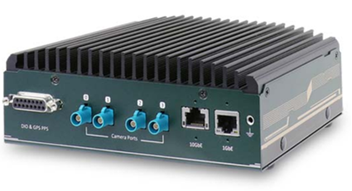
\includegraphics[width=0.55\textwidth]{figures/template/nru51v_photo.png}
  \caption{The Neousys NRU-51V (NVIDIA Jetson Xavier NX), showing the four
  FAKRA camera ports.}
  \label{fig:nru51v-photo}
\end{figure}

\begin{figure}[htbp]
  \centering
  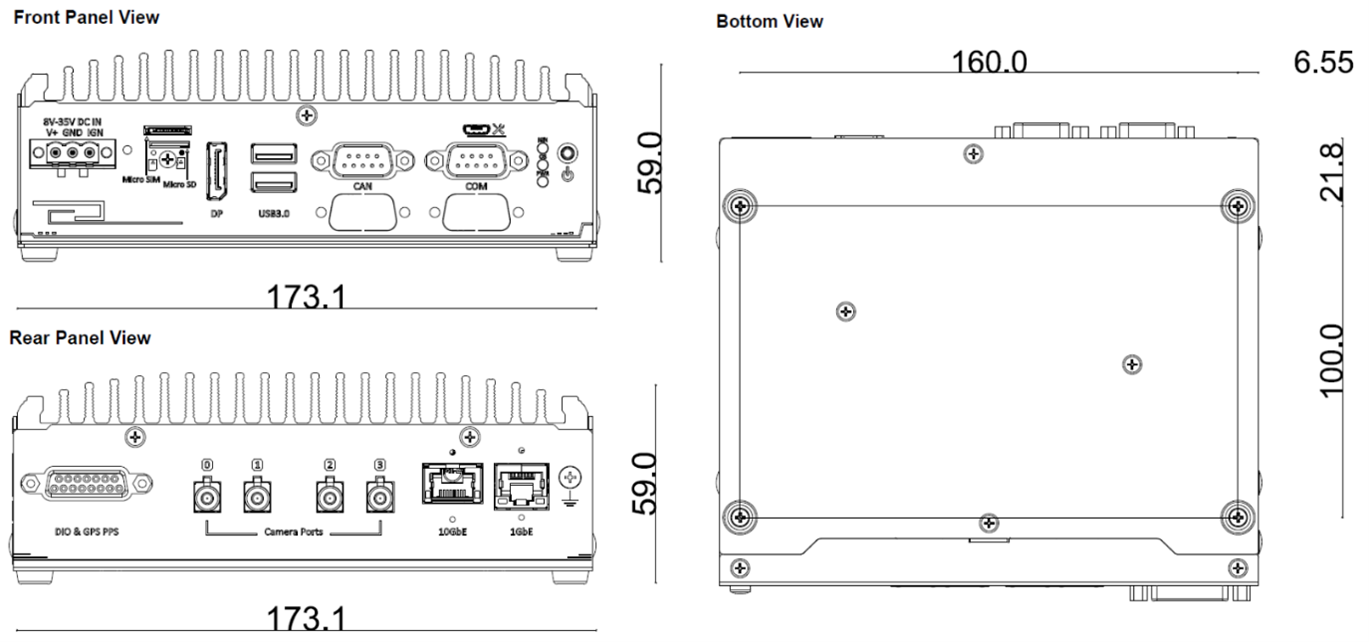
\includegraphics[width=\textwidth]{figures/template/nru51v_dimensions.png}
  \caption{Dimensions of the Neousys NRU-51V in millimetres.}
  \label{fig:nru51v-dimensions}
\end{figure}

\begin{table}[htbp]
\centering
\caption{Summary of the hardware technical specification.}
\label{tab:hardware-spec}
\small
\begin{tabularx}{\textwidth}{>{\raggedright\arraybackslash}p{0.22\textwidth}>{\raggedright\arraybackslash}p{0.34\textwidth}>{\raggedright\arraybackslash}X}
\toprule
Device / sensor & Model / specification & Role in the system \\
\midrule
Edge processing unit & Neousys NRU-51V (NVIDIA Jetson Xavier NX, 21~TOPS) &
  runs YOLO26, the SLAM system and the ROS~2 navigation stack \\
Stereo camera module & AC-IMX390-H190 (Sony IMX390 sensor) & records
  \SI{186}{\degree} stereo imagery for object detection and feature
  extraction \\
Inertial sensor (IMU) & 6-DoF industrial IMU (\SIrange{100}{200}{\hertz}) &
  measures acceleration and angular rate to support pose estimation (VIO) \\
Mobile testbed & AMR platform (speed \SI{1.5}{\metre\per\second}, slope
  \SI{5}{\degree}) & robot base for online navigation tests in the mock
  environment \\
\bottomrule
\end{tabularx}
\end{table}

\subsection{Real sensor rig and calibration limits}
\label{sec:real-calibration}
% Verbatim from minor_report/chapters/chapter_3_methodology.tex lines 534-573 (retired report),
% headings demoted by 0 level(s). Do not edit here; edit the source of the numbers.

The real configuration is summarised in \cref{tab:real-rig}. Its calibration is
materially weaker than the simulated rig's, and the weaknesses are load bearing
rather than cosmetic.

\begin{table}[htbp]
\centering
\caption[Real sensor rig, and the calibration status of each quantity.]{Real sensor rig, and the calibration status of each quantity. Only the
first three rows are measured; the remainder are approximations or placeholders
that bound what can be claimed from real-robot data.}
\label{tab:real-rig}
\small
\begin{tabularx}{\textwidth}{>{\raggedright\arraybackslash}p{0.26\textwidth}>{\raggedright\arraybackslash}p{0.30\textwidth}>{\raggedright\arraybackslash}X}
\toprule
Quantity & Value & Status \\
\midrule
Stereo resolution & $1920\times1080$ fisheye & measured \\
Stereo baseline & \SI{0.093604}{\metre} & measured \\
IMU stream & \repo{/hwt101ct_yaw_publisher} & separate RealSense source \\
Camera model (ORB-SLAM3) & \texttt{KannalaBrandt8} & configured \\
Camera model (VINS) & project fisheye files & configured \\
Second-camera intrinsics & reuse of the first camera & \flag{approximation} \\
IMU-to-camera rotation & observational support & partial \\
IMU-to-camera translation & zero & \flag{placeholder} \\
Stationary $\lVert a\rVert$ & \SI{9.2642}{\metre\per\second\squared} &
  \flag{measured, deviates from \num{9.81}} \\
Extrinsic estimation (VINS) & \repo{estimate_extrinsic: 1} & online \\
Time-offset estimation (VINS) & \repo{estimate_td: 1} & online \\
\bottomrule
\end{tabularx}
\end{table}

The real IMU-to-camera rotation has observational support, but its translation is
a zero placeholder. The stationary accelerometer magnitude is recorded as
\SI{9.2642}{\metre\per\second\squared}, rather than
\SI{9.81}{\metre\per\second\squared}. VINS-Fusion uses the observed magnitude as
\repo{g_norm}; the ORB-SLAM3 real inertial launch rescales acceleration by
$9.81/9.2642$. These treatments make the configurations internally consistent but
do not replace an independent camera--IMU calibration. Real trajectories can be
inspected for plausibility and tracking continuity, but metric accuracy cannot be
claimed without independent ground truth and improved extrinsic calibration.


\subsection{Test site and experimental variables}
\label{sec:real-site}

\textbf{Spatial layout.} The test area is divided into two operating zones,
Zone~A and Zone~B, separated by and connected through a walkway (each zone
about \SI{3}{\metre} square, walkway \SI{1.25}{\metre} wide;
\cref{fig:test-field}). The division reproduces the traffic pattern of a
warehouse AMR that shuttles continuously between a pick-up and a drop-off
point. The robot's linear speed is limited to $v_{\max} =
\SI{1.5}{\metre\per\second}$ throughout.

\textbf{Ground truth by motion capture.} Evaluating SLAM error (ATE and RPE)
needs a reference accurate to millimetres. A motion-capture camera system is
installed around the test area and tracks reflective markers placed at the
robot's centre of mass at a rate above \SI{100}{\hertz}.

\textbf{Coordinate-frame alignment.} The SLAM pose $P_{\mathrm{slam}}$ is
expressed in the local odometry frame fixed at start-up, whereas the
motion-capture pose $P_{\mathrm{gt}}$ is expressed in the room's global frame.
Before errors are computed the two trajectories are aligned by a rigid-body
transformation; the alignment actually used for every result in this report,
and its treatment of scale, is defined in \cref{sec:method-trajectory}.

\textbf{Dynamic-environment variable.} Each time the robot completes a zone
transfer (for example arrives in Zone~B from Zone~A), the operator randomly
re-positions and re-counts the stacks of goods in the opposite zone before the
robot returns. This forces the SLAM system to face a scene that no longer
matches its map (map obsolescence), to test whether ORB-SLAM3's Atlas or
RTAB-Map's memory management can resolve the conflicting spatial evidence
without tracking loss.

\textbf{Illumination variable.} Data are collected along the same route at
three times of day representing different light levels and directions:
morning (08:00), oblique natural light casting shadows across the test area;
midday (12:00), maximum brightness, with possible high contrast or
over-exposure in places; and evening (18:00), low light relying mainly on the
building's artificial lighting, with raised image noise. The variable tests
both the camera hardware (Sony IMX390 HDR) and the robustness of the two SLAM
frameworks in keeping enough inlier features for odometry under variable light.

\textbf{Real-dataset status.} Three real recordings exist
(\cref{tab:dataset-registry}). Only \repo{dataset_real_000} carries inertial
data; \repo{dataset_real_001} and \repo{_002} contain zero IMU messages and
support image-only work at most. No real recording carries motion-capture
ground truth or wheel odometry at the cutoff, which is why every real-robot
result slot in \cref{chap:results} is planned rather than filled.

\section{The Four Experiments}
\label{sec:experiments}

Each experiment below is defined by its objective, its process, its evaluation
metrics, its constraints and the validity rule that decides whether a run
counts. Each is run in both domains; \cref{chap:results} reports each domain in
its own slot.

\subsection{Experiment 1: Non-visual baseline and estimator comparison}
\label{sec:proprio-method}

\textbf{Objective.} Establish a dead-reckoning baseline to determine whether the
visual pipelines (ORB-SLAM3 and VINS-Fusion) genuinely outperform the robot's
own wheel odometry, its IMU, and a wheel-plus-IMU extended Kalman filter, and
whether the uncertainty each estimator reports describes the error it makes.

\textbf{Process.} Wheel odometry, IMU dead reckoning and the EKF are run
offline on the same recordings the visual estimators consumed, from
proprioceptive topics only. A calibration pass measures each sensor's noise and
scale against ground truth first; the estimators then run and are scored on the
same interval as the visual runs.

\textbf{Evaluation metrics.} Aligned and anchored ATE, final drift as a fraction
of distance, final heading error, RPE at \SI{1}{\second}, and the covariance
consistency measures NEES and $k\sigma$ coverage.

\textbf{Validity rule.} A run counts only if the planar assumption holds
(maximum tilt below \SI{1}{\degree}), the IMU orientation field is not consumed,
and the number of wheel corrections equals the number of wheel-odometry
messages.

% Verbatim from minor_report/chapters/chapter_3_methodology.tex lines 1263-1478 (retired report),
% headings demoted by 1 level(s). Do not edit here; edit the source of the numbers.

The visual estimators were, until the cutoff, scored only against ground truth.
That establishes how large their error is but not whether it is good, because no
alternative was measured on the same data. Three non-visual estimators were
therefore implemented in \repo{script/proprio_estimator.py} to supply a
dead-reckoning floor: wheel odometry, IMU dead reckoning, and an extended Kalman
filter fusing the two. They consume only proprioceptive topics and no images.

\subsubsection{Implementation form and why it is offline}

All three read the recorded bag directly and are deterministic functions of it.
Run as live ROS nodes they would instead depend on replay rate, QoS delivery and
CPU contention, none of which is a property of the estimator being compared. The
cost is a stated asymmetry: the visual figures they are compared against were
produced by live runs, so any timing-induced error is present on one side of the
comparison only. This is revisited in \cref{sec:results-proprio}.

\subsubsection{Sensor model derived from data}

Every covariance field in the source bags is identically zero---0 of 17\,416 IMU
messages, 0 of 4\,355 wheel-odometry messages, and 0 of 4\,354 ground-truth
messages in \repo{dataset_allsensor_000}. Gazebo Fortress does not populate them,
and \texttt{AckermannSteering} exposes no noise parameter. The noise model is
consequently measured rather than read, by a \repo{calibrate} step that writes
\repo{sensor_noise.yaml}; \cref{tab:proprio-noise} gives the result for both bags.

\begin{table}[htbp]
\centering
\caption[Sensor noise and scale measured from each bag by \repo{proprio_estimator.py calibrate}.]{Sensor noise and scale measured from each bag by
\repo{proprio_estimator.py calibrate}. Scales are least-squares gains through the
origin against ground truth; $\sigma$ values are the residual standard deviations.
A scale of 1.0 is an unbiased sensor. The bias random walks are assumed, not
measured, because the longest stationary window is \SI{1.54}{\second}.}
\label{tab:proprio-noise}
\small
\resizebox{\textwidth}{!}{%
\begin{tabular}{llrrrrrl}
\toprule
Group & Quantity & \repo{_000} & \repo{_001} & \repo{_002} & \repo{_003} &
  \repo{_004} & Units \\
 & & plain & plain & plain & bayline & bayline & \\
\midrule
IMU & gyroscope $z$ bias & $6.48\times10^{-5}$ & $7.75\times10^{-5}$ &
  $9.28\times10^{-5}$ & $6.09\times10^{-4}$ & $2.58\times10^{-5}$ & \si{\radian\per\second} \\
 & gyroscope $\sigma$ & $4.36\times10^{-3}$ & $4.24\times10^{-3}$ &
  $4.81\times10^{-3}$ & $5.03\times10^{-3}$ & $5.15\times10^{-3}$ & \si{\radian\per\second} \\
 & gyroscope $z$ scale & 0.9990 & 1.0000 & 1.0002 & 1.0002 & 1.0000 & -- \\
 & accelerometer $x$ bias & 0.0191 & 0.0304 & \flag{0.0683} & 0.0309 & 0.0016 &
  \si{\metre\per\second\squared} \\
 & accelerometer $x$ scale & 1.0199 & 1.0249 & \flag{1.0669} & \flag{1.0525} & \flag{1.0465} & -- \\
 & measured $g$ & 9.7809 & 9.8191 & 9.7827 & 9.8037 & 9.8346 & \si{\metre\per\second\squared} \\
\midrule
Wheel & speed scale & 1.0002 & 0.9985 & 1.0005 & 1.0071 & 1.0001 & -- \\
 & speed $\sigma$ & 0.0407 & 0.0484 & 0.0496 & 0.0607 & 0.0505 & \si{\metre\per\second} \\
 & yaw-rate scale, bicycle & 1.0110 & 0.9527 & 1.0034 & \flag{0.9375} & \flag{0.9250} & -- \\
 & yaw-rate $\sigma$, bicycle & 0.0659 & 0.0804 & 0.0705 & 0.1192 & 0.0613 &
  \si{\radian\per\second} \\
 & yaw-rate scale, differential & 1.2162 & 1.1442 & 1.2194 & 1.2748 & 1.1404 & -- \\
 & yaw-rate $\sigma$, differential & 0.2359 & 0.3074 & 0.2620 & 0.3477 & 0.2828 &
  \si{\radian\per\second} \\
\midrule
Window & static duration & 0.68 & 0.58 & 1.54 & 1.04 & \flag{0.52} & \si{\second} \\
 & maximum tilt & 0.0016 & 0.0018 & 0.0015 & 0.0018 & 0.0017 & \si{\degree} \\
\bottomrule
\end{tabular}}
\end{table}

Two consequences follow directly. First, wheel \emph{speed} is essentially
unbiased on all five bags (scale 1.0002 to 1.0071), so distance travelled is not
the error source. Second, the rear-wheel differential is a far worse yaw-rate estimator
than the steering-angle bicycle model---residuals of \SIrange{0.26}{0.35}{\radian\per\second}
against \numrange{0.061}{0.119}---because the track
and the wheel base are both \SI{0.42}{\metre} and a solid rear axle slips through
every turn. The bicycle model is selected automatically and was chosen on all five
bags.

\subsubsection{The orientation field must not be used}

\texttt{sensor\_msgs/Imu.orientation} in these bags is not an estimate. Measured
over \repo{dataset_allsensor_000} it equals ground-truth yaw minus exactly
\SI{90}{\degree}, with residual standard deviation \SI{0.00000}{\degree} and
\SI{0.00000}{\degree} of drift across \SI{87}{\second}: the plugin publishes the
true orientation from the simulator's entity-component manager. Consuming it
would give a ``dead-reckoning'' estimator a perfect attitude reference that no
real IMU has, and its output would measure ground truth. All three estimators
therefore integrate \texttt{angular\_velocity.z} instead, which drifts honestly by
\SI{2.52}{\degree} over \SI{87}{\second} on \repo{allsensor_000} and
\SI{1.70}{\degree} over \SI{81.8}{\second} on \repo{allsensor_001}. The same check
on \repo{allsensor_002} again returns a residual standard deviation of
\SI{0.000000}{\degree} against ground-truth yaw, so the exclusion is not specific
to the first two recordings. Each run
records \repo{imu_orientation_used=NO} in its metadata so the exclusion is
auditable.

\subsubsection{Estimator definitions}

\Cref{tab:proprio-estimators} defines the three estimators. The EKF carries the
planar state $\mathbf{x}=[p_x,p_y,\theta,v,b_\omega]^{\top}$, predicted at the
\SI{200}{\hertz} IMU rate and corrected at \SI{50}{\hertz} by the wheels.

\begin{table}[htbp]
\centering
\caption[Implemented non-visual estimators.]{Implemented non-visual estimators. ``Anchoring'' refers to the initial
pose: dead reckoning has no global reference, so all three start from the
ground-truth pose at their first sample, and this is recorded as an alignment
decision rather than treated as neutral.}
\label{tab:proprio-estimators}
\small
\begin{tabularx}{\textwidth}{>{\raggedright\arraybackslash}p{0.15\textwidth}>{\raggedright\arraybackslash}p{0.21\textwidth}>{\raggedright\arraybackslash}p{0.21\textwidth}>{\raggedright\arraybackslash}X}
\toprule
Estimator & Inputs & State & Correction \\
\midrule
Wheel odometry & rear wheel speeds, steering angles (\SI{1}{\kilo\hertz}) &
  $[p_x,p_y,\theta]$ & none; $\mathbf{P}$ grows without bound \\
IMU dead reckoning & gyroscope $z$, accelerometer $x$ (\SI{200}{\hertz}) &
  $[p_x,p_y,\theta,v]$ & none \\
EKF wheel + IMU & both of the above & $[p_x,p_y,\theta,v,b_\omega]$ & wheel speed
  corrects $v$; $(\omega_{\text{gyro}}-\omega_{\text{wheel}})$ corrects
  $b_\omega$ \\
\bottomrule
\end{tabularx}
\end{table}

\subsubsection{EKF formulation}
\label{sec:ekf-formulation}

\paragraph{State and inputs.} The filter carries five planar states,
\begin{equation}
  \mathbf{x} = \begin{bmatrix}p_x & p_y & \theta & v & b_\omega\end{bmatrix}^{\top},
  \label{eq:ekf-state}
\end{equation}
where $b_\omega$ is the gyroscope $z$ bias. Roll and pitch stay within
\SI{0.002}{\degree} across every recording, so a full 15-state inertial
formulation would spend nine states on quantities this platform does not have,
and their covariances would be unobservable noise in the consistency test that
motivates the experiment.

The IMU is not a measurement here: it drives the prediction. Bias-corrected yaw
rate and longitudinal acceleration act as the input,
\begin{equation}
  \omega = \omega_{\text{gyro}} - b_\omega, \qquad a = a_x - b_a,
  \label{eq:ekf-input}
\end{equation}
with $b_a$ a constant measured during calibration rather than a tracked state.
Propagation uses the midpoint heading $\theta_m = \theta + \tfrac{1}{2}\omega\,\Delta t$,
which matters over \SI{117}{\metre} of driving:
\begin{align}
  p_x &\mathrel{+}= v\cos\theta_m\,\Delta t + \tfrac{1}{2}a\cos\theta_m\,\Delta t^2, \notag\\
  p_y &\mathrel{+}= v\sin\theta_m\,\Delta t + \tfrac{1}{2}a\sin\theta_m\,\Delta t^2, \notag\\
  v   &\mathrel{+}= a\,\Delta t, \qquad \theta \mathrel{+}= \omega\,\Delta t.
  \label{eq:ekf-propagate}
\end{align}

\paragraph{Covariance and process noise.} With $\mathbf{F}=\partial f/\partial
\mathbf{x}$ and $\mathbf{G}$ mapping the noise inputs into the state,
\begin{equation}
  \mathbf{P} \leftarrow \mathbf{F}\mathbf{P}\mathbf{F}^{\top}
    + \mathbf{G}\,\mathrm{diag}(\sigma_a^2,\ \sigma_g^2,\ \sigma_{b}^2)\,\mathbf{G}^{\top}.
  \label{eq:ekf-predict}
\end{equation}
The non-trivial entries are
$F_{13}=-v\sin\theta_m\Delta t$, $F_{14}=\cos\theta_m\Delta t$,
$F_{23}=v\cos\theta_m\Delta t$, $F_{24}=\sin\theta_m\Delta t$ and
$F_{35}=-\Delta t$; the last couples bias error directly into heading, which is
what makes $b_\omega$ worth estimating. In $\mathbf{G}$, accelerometer noise
enters position as $\tfrac{1}{2}\cos\theta_m\Delta t^2$ and speed as $\Delta t$,
gyroscope noise enters heading as $\Delta t$, and the bias row carries
$\sqrt{\Delta t}$ rather than $\Delta t$ because a random walk accumulates as
$\sqrt{t}$.

Both IMU noise terms are therefore \emph{process} noise. Nothing from the IMU
appears in $\mathbf{R}$, because the IMU propagates the state rather than
observing it.

\paragraph{Measurement.} The wheels correct at \SI{50}{\hertz} with
\begin{equation}
  \mathbf{z} = \begin{bmatrix}v_{\text{wheel}} \\
    \omega_{\text{gyro}} - \omega_{\text{wheel}}\end{bmatrix}, \qquad
  \mathbf{H} = \begin{bmatrix}0&0&0&1&0\\ 0&0&0&0&1\end{bmatrix}, \qquad
  \mathbf{R} = \mathrm{diag}\!\left(\sigma_{v,w}^2,\ \sigma_{\omega,w}^2+\sigma_g^2\right).
  \label{eq:ekf-update}
\end{equation}
The second variance is a sum because that observation is a \emph{difference} of
two noisy sensors and inherits both. The update uses the Joseph form,
\begin{equation}
  \mathbf{P} \leftarrow (\mathbf{I}-\mathbf{K}\mathbf{H})\mathbf{P}
    (\mathbf{I}-\mathbf{K}\mathbf{H})^{\top} + \mathbf{K}\mathbf{R}\mathbf{K}^{\top},
  \label{eq:ekf-joseph}
\end{equation}
symmetrised afterwards. The shorter $(\mathbf{I}-\mathbf{K}\mathbf{H})\mathbf{P}$
does not reliably stay positive definite across the roughly \num{16000} updates
in a run, and here the covariance is itself the measurement under test, so it
cannot be allowed to decay.

\paragraph{Where the numbers come from.} $\sigma_a$ and $\sigma_g$ are measured
from the recording by the calibration pass (\cref{tab:proprio-noise}), not taken
from a datasheet, because every covariance field in these bags is identically
zero. $\sigma_{v,w}$ and $\sigma_{\omega,w}$ likewise come from the wheel stream
against ground truth. \moved{$\sigma_b$, the bias random walk, is assumed rather
than measured: the longest stationary window in any recording is
\SI{1.54}{\second} and an Allan-variance estimate needs minutes.}

\subsubsection{Why the bias, and not the heading, is observed}

The EKF's second measurement is deliberately an observation of the \emph{gyroscope
bias} and not of heading. Integrating the wheel yaw rate into a heading and
correcting $\theta$ with it would reproduce the wheel estimator inside the filter
and inherit its unbounded drift. Treating the instantaneous rate difference as an
observation of $b_\omega$ keeps each sensor supplying what it measures well: the
wheels know rate, the gyroscope knows change, and neither knows absolute heading,
so heading remains unobservable and its variance correctly continues to grow. The
update uses the Joseph form, which keeps $\mathbf{P}$ symmetric and positive
definite across the roughly 16\,000 updates in a run.

Measured scale errors are recorded but never divided out. Correcting them would
mean calibrating the estimator with the ground truth it is about to be scored
against; the scale error is a real property of encoder odometry and is retained.


\subsection{Experiment 2: Offline YOLO detector performance}
\label{sec:yolo-eval-method}

\textbf{Objective.} Measure standalone detector performance independent of
SLAM, so that later filtering results can be attributed: how reliably the
detector finds and names warehouse objects, and how much of the frame a mask
built from its boxes would remove.

\textbf{Process.} The detector is run on every left-camera frame of the dynamic
recordings; ground-truth boxes are constructed by projecting the simulator's
own object geometry into the camera; predictions are matched by class at an IoU
threshold; localization and class assignment are scored separately.

\textbf{Evaluation metrics.} Precision, recall, F1, recall on the moving subset,
image-area coverage, and conditional class precision, recall and F1.

\textbf{Validity rule.} Overlays are inspected before any aggregate is
accepted, because invalid pose stamps, mesh units or camera transforms produce
plausible but wrong boxes.

% Verbatim from minor_report/chapters/chapter_3_methodology.tex lines 1655-1772 (retired report),
% headings demoted by 1 level(s). Do not edit here; edit the source of the numbers.

Detector precision, recall, TP, FP, FN, moving/static recall, IoU, and image-area
coverage are computed by \repo{yolo_eval.py} at recorded confidence, matching-IoU,
occlusion, minimum-size, and motion thresholds. Mask-use statistics are joined to
trajectories by \repo{timestamp_ns}. A semantic class is never treated as
ground-truth motion.

\paragraph{Constructing the ground-truth boxes} 
\label{sec:yolo-gt-projection}

The detector is scored against boxes computed from the simulator's own state
rather than against hand annotation. No image is labelled by hand anywhere in
this project. The chain from a recorded object pose to a box in pixels is as
follows; all of it is in \repo{yolo_eval.py} and \repo{yolo_gt.py}.

\begin{enumerate}[leftmargin=1.6em]
  \item \textbf{Geometry, not just pose.} A pose is a point and a box needs
    extent, so \repo{yolo_gt.vertices()} reads the prop's collision mesh
    (\repo{.dae}) from the Gazebo model directory and returns its vertices
    $V$ in the model frame. Meshes above \num{4000} vertices are decimated with
    a fixed seed: a few thousand points bound a silhouette as tightly as
    \num{100000} and keep the per-frame cost flat.
  \item \textbf{Object to world.} The pose $(R_{wo}, p_{wo})$ recorded for that
    object places the vertices: $v_w = R_{wo} V + p_{wo}$.
  \item \textbf{Camera pose.} The robot pose gives $T_{wb}$, and the camera is
    placed on the body by the extrinsic $T_{bc}$ read from
    \repo{config/wil_sim/stereo_imu.yaml}, so $T_{wc} = T_{wb} T_{bc}$. Reading
    the extrinsic from the estimator's own configuration file is deliberate: the
    evaluation and VINS-Fusion then cannot disagree about where the camera is.
  \item \textbf{World to camera}, by inverting that transform, using the
    transpose because the rotation is orthonormal:
    $R_{cw} = R_{wc}^{\top}$, $t_{cw} = -R_{cw} t_{wc}$, $v_c = R_{cw} v_w +
    t_{cw}$.
  \item \textbf{Projection.} Vertices with $z \le \SI{0.05}{\metre}$ are
    discarded \emph{before} the division, then the remainder are projected
    through an ideal pinhole:
    \begin{equation}
      u = f_x \frac{x_c}{z_c} + c_x, \qquad
      v = f_y \frac{y_c}{z_c} + c_y .
      \label{eq:pinhole}
    \end{equation}
  \item \textbf{Box.} The axis-aligned extent of the projected points,
    $[\min u, \max u] \times [\min v, \max v]$, clipped to the image.
\end{enumerate}

The $z$ guard in step 5 is not a formality. A vertex behind the camera has
negative $z$, and the division then mirrors it to the wrong side of the image,
producing a well-formed box in entirely the wrong place --- a failure that looks
like a detector error rather than a projection error. Objects that straddle the
image plane are projected from their visible vertices only.

Each object also stores $\tilde{z} = \mathrm{median}(z_c)$, which is what the
occlusion test below uses to decide which of two overlapping objects is nearer.

\begin{table}[htbp]
\centering
\caption[Parameters of the detection evaluation.]{Parameters of the detection evaluation. The intrinsics are not
calibrated: Gazebo renders an ideal pinhole, so $f_x = f_y = (W/2)/\tan(\phi/2)$
with every distortion term zero, and the values below are exact rather than
estimated. The three exemption rules decide which ground-truth objects are scored
at all, and are the reason the recall in \cref{sec:yolo-performance} is computed
over a subset of the objects present.}
\label{tab:yolo-eval-params}
\small
\begin{tabularx}{\textwidth}{>{\raggedright\arraybackslash}p{0.30\textwidth}lX}
\toprule
Parameter & Value & Role \\
\midrule
$f_x$, $f_y$ & \num{640}, \num{640} & ideal pinhole, \SI{90}{\degree} horizontal
  field of view \\
$c_x$, $c_y$ & \num{640}, \num{360} & principal point at image centre \\
Image size & $1280 \times 720$ & \\
Distortion & all zero & the renderer applies none \\
Mesh vertices per prop & $\le \num{4000}$ & decimated with a fixed seed \\
Near-plane guard & \SI{0.05}{\metre} & vertices nearer than this are dropped
  before projection \\
\midrule
Confidence, \repo{--conf} & \num{0.35} & detections below this are never emitted \\
NMS IoU, \repo{--iou-nms} & \num{0.5} & \\
Matching IoU, \repo{--iou-match} & \num{0.5} & prediction counts as a hit above
  this \\
Motion threshold, \repo{--move-thresh} & \SI{0.05}{\metre\per\second} & object
  is ``moving'' above this, from its pose history \\
\midrule
\textbf{Exemption:} minimum size, \repo{--min-box-px} & \SI{12}{px} & smaller
  ground-truth boxes are discarded and never appear \\
\textbf{Exemption:} occlusion, \repo{--occlusion} & \num{0.70} & ground truth
  covered more than this by nearer objects is scored as neither hit nor miss
  (\emph{yellow} in \cref{fig:yolo-ground-truth-overlay}) \\
\textbf{Exemption:} scenery cover, \repo{--ignore-cover} & \num{0.50} & a
  prediction this covered by unlabelled scenery is neither credited nor penalised \\
\bottomrule
\end{tabularx}
\end{table}

\paragraph{What this convention costs} 

Two consequences follow from scoring against projected geometry, and both bear on
how the detector numbers in \cref{sec:yolo-performance} should be read.

The boxes are \emph{tighter than a human would draw}. They are the exact
silhouette of the collision mesh, whereas an annotator draws a looser rectangle
and rounds generously. A detector trained on human boxes is therefore scored
against a stricter convention than it was fitted to, and loses IoU that
represents no error on its part. Of the differences between how this detector
is scored here and how it was scored during training, this is the one that cannot
be removed without relabelling.

The exemptions are \emph{not symmetric with the training convention}. A
human-annotated set has no notion of an exempt object: every labelled box counts.
The occlusion and minimum-size rules exist because a crate that is nine tenths
behind a shelf is not a fair test of a detector, which is the right decision for
reporting detector quality --- but it means recall here is computed over the
easier subset. The size of that effect is measurable from the stored counts:
\num{34476} of the \num{96758} ground-truth objects across the five recordings
are exempt, and recomputing recall with every one of them counted as a miss moves
it from \num{0.593} to \num{0.382}
(\repo{script/yolo_generalization.py}). Any comparison against a
training-set recall has to use the second figure, not the first.


\subsection{Experiment 3: Visual-inertial odometry with dynamic-environment
filtering}
\label{sec:vio-filter-method}

\textbf{Objective.} Determine whether masking dynamic-object features improves
localization, measure the compute cost of doing so, and verify that tracking
survives the filtering and that the added detector cost does not push either
pipeline below the input frame rate.

\textbf{Process, simulation.} Each visual pipeline is run on each recording in
two treatments, baseline and filtered, as separate processes on identical
input, three repeats per condition. The treatment pair is valid only when the
filter demonstrably acted (matched detections, non-zero mask coverage, removed
tracks) and the two runs received the same input to within \SI{5}{\percent} in
image count and duration. The collection protocol is given in
\cref{sec:collection-validity}.

\textbf{Process, real robot (planned).} The online procedure has four steps.
\emph{Step~1, initialisation and time synchronisation:} power the NRU-51V, the
stereo cameras and the IMU; start the motion-capture system and calibrate the
room; synchronise the ROS~2 clock on the robot with the motion-capture server by
PTP or Chrony (NTP), since a fraction of a second of offset corrupts ATE and
RPE. \emph{Step~2, execution and environment alteration:} drive from the origin
in Zone~A to the goal in Zone~B at a linear speed not above
\SI{1.5}{\metre\per\second} through the Nav2 package; on arrival, trigger the
dynamic variable by randomly re-placing the $k$ stacks in Zone~A; return, alter
Zone~B, and alternate for five minutes per test cycle to represent a
lifelong-mapping load. \emph{Step~3, data logging:} record with rosbag2 the
6-DoF SLAM pose, the motion-capture reference, the detector boxes with
confidences, and the whole-pipeline latency per frame. \emph{Step~4, iteration
over the experimental matrix:} repeat steps 1--3 for both pipelines under the
three illumination levels. The \texttt{.db3} bags are then trajectory-extracted
and timestamp-matched before evaluation.

\textbf{Evaluation metrics.} ATE and rotational RMSE after rigid alignment,
RPE at $\Delta = \SI{1}{\second}$ (all pairs and jump-free), tracking-loss and
reset events, retained input fraction, throughput, process CPU and peak memory,
and per-module latency against the inter-frame budget.

\textbf{Validity rule.} A trajectory containing steps that imply more than
\SI{10}{\metre\per\second} is not read as ordinary drift; an indoor error above
\SI{50}{\metre} is divergence. A comparison across treatments is admissible only
for input-matched pairs with an active filter.

\subsection{Experiment 4: Dense map reconstruction and map-quality evaluation}
\label{sec:map-eval-method}

\textbf{Objective.} Verify whether the reconstructed map accurately reflects the
physical environment and is usable by a route planner.

\textbf{Process.} RTAB-Map builds a database from a mapping run; the occupancy
grid is seated in the world by a fixed transform measured from the map alone;
geometry is scored against the world's collision meshes; drivability is scored
by stamping the true robot footprint along a ground-truth route that did not
build the map.

\textbf{Evaluation metrics.} Occupied-cell precision, recall over observed
surfaces and over the whole building, false-obstacle rate under the footprint,
unmapped footprint poses, clearance statistics, and the graph's node and link
counts.

\textbf{Validity rule.} Placement must be established independently before any
metric is read, and a drivability figure computed against the run that built
the map is a self-consistency check, not a result.

% Verbatim from minor_report/chapters/chapter_3_methodology.tex lines 1776-1795 (retired report),
% headings demoted by 0 level(s). Do not edit here; edit the source of the numbers.

RTAB-Map grids are placed in the Gazebo world using one fixed rigid world-to-map
transform measured by \repo{script/fit_map_pose.py}. It is constant for a database;
the live \texttt{map~$\rightarrow$~odom} drift correction is not reused for map
placement.

\repo{script/validate_map.py} rasterizes world collision geometry and evaluates
occupied cells at a stated tolerance. It reports occupied-cell precision,
whole-world and observed-region recall, false obstacles under the true
$0.83\times0.50$~m footprint, unmapped footprint poses, and clearance. Graph
evaluation records neighbour, global-closure, local-space, and gravity links.
Localization additionally requires time to first fix, accepted and rejected
matches, database checksums before and after read-only operation, pose continuity,
and known-world bounds. Finite covariance or a localization status message alone
does not establish correctness.

At the cutoff this evaluation has been applied to one database,
\repo{map/map_tiny.db}, against
\repo{small_warehouse_static/small_warehouse_static_tinymap.world}. The
equivalent large-warehouse evaluation is \status{planned} and no database for
it exists; results are reported in \cref{sec:map-quality}.


\section{Evaluation Metrics and Analysis}
\label{sec:evaluation-method}

\subsection{Trajectory evaluation}
\label{sec:method-trajectory}
% Verbatim from minor_report/chapters/chapter_3_methodology.tex lines 1590-1651 (retired report),
% headings demoted by 0 level(s). Do not edit here; edit the source of the numbers.

\repo{script/vio_metrics.py} associates estimate and reference over their common
time interval and interpolates the reference at estimator timestamps. A rigid
Umeyama $SE(3)$ fit maps estimated positions to the reference with scale fixed at
one. Fixed scale is appropriate for stereo-inertial estimators and preserves
scale error. Outputs include translational ATE RMSE, maximum and final error,
rotational geodesic error, path length, overlap duration, pose count, jump count,
and longest jump-free segment. Optional startup trimming is relative to each
estimator's first overlapping pose, preventing unequal initialization latency
from being interpreted as steady-state behaviour.

The older \repo{plot_vio_vs_gt.py} provides a first-pose-aligned diagnostic, but
headline comparison uses common $SE(3)$ alignment. Real data without independent
ground truth receives no ATE.

\paragraph{Relative pose error.} RPE was added to \repo{script/vio_metrics.py}
after the reporting cutoff, on 18 September 2026, and is
\status{implemented and exercised on the full campaign}. It follows the
conventional definition: for a pair of poses separated by a fixed interval
$\Delta$, the error transform is
\begin{equation}
  E_i = \left(Q_i^{-1}Q_{i+k}\right)^{-1}\left(P_i^{-1}P_{i+k}\right),
  \label{eq:rpe}
\end{equation}
with $P$ the estimate and $Q$ the reference. Translational RPE is
$\lVert\operatorname{trans}(E_i)\rVert$ and rotational RPE is the geodesic angle
of $\operatorname{rot}(E_i)$, the same angle measure used for orientation error
above.

RPE is reported because it needs \emph{no} global alignment, and that is what
makes it the appropriate metric for the dynamic runs. A single discontinuity
re-seats the rigid $SE(3)$ fit, so every subsequent pose inherits the offset and
ATE describes the jump rather than the tracking. RPE instead asks a local
question --- over the next $\Delta$ seconds, did the estimate move as the
reference moved --- and is insensitive to both the global frame and accumulated
drift. It therefore supersedes the longest-jump-free-segment statistic, which
answers a similar question through a segment-selection heuristic rather than a
standard definition.

Four intervals are swept, $\Delta \in \{0.5, 1, 2, 5\}\,\si{\second}$, giving
an error-versus-interval curve; $\Delta = \SI{1}{\second}$ is the headline value
and corresponds to roughly \SI{1.4}{\metre} at the simulated robot's cruising
speed. A pair is admitted only when its realised separation lies within
\SI{25}{\percent} of $\Delta$, so a gap in the log cannot silently widen the
interval and inflate the error; the surviving pair count is reported with every
statistic. Pairs are overlapping, which is the conventional default.

Each statistic is computed twice: over all admissible pairs, and over only those
pairs that do not span a detected tracking jump. The difference isolates the
teleport contribution from ordinary local error, mirroring the existing
separation between global and clean-segment ATE. Both RMSE and median are
reported, because the dynamic-run distributions are strongly right-skewed and a
single teleport otherwise sets the RMSE.

The implementation is verified against synthetic trajectories with known answers:
an estimate identical to the reference returns zero; a constant relative drift of
\SI{0.1}{\metre\per\second} returns \SI{0.100}{\metre} at
$\Delta=\SI{1}{\second}$ and \SI{0.200}{\metre} at $\Delta=\SI{2}{\second}$; a
\SI{2}{\degree\per\second} relative rotation returns \SI{2.00}{\degree} at
$\Delta=\SI{1}{\second}$; and an injected teleport separates the all-pairs and
jump-free statistics by the expected pair count. Results are written to
\repo{rpe_metrics.csv} for the interval sweep, with the
$\Delta=\SI{1}{\second}$ values carried into \repo{trajectory_metrics.csv}.


\subsection{Computational performance}
% Verbatim from minor_report/chapters/chapter_3_methodology.tex lines 1799-1811 (retired report),
% headings demoted by 0 level(s). Do not edit here; edit the source of the numbers.

Both estimator processes write per-frame \repo{performance.csv} files. These
record processing time, delivery and backlog counters, tracking or solver state,
initialization and reset evidence, pose and keyframe accounting, cumulative
process CPU time, monotonic wall time, and resident memory. VINS additionally
records feature-front-end and estimator-back-end stages; ORB-SLAM3 records its
tracking front end, local mapping, place recognition, loop closure, map merging,
and global bundle-adjustment events. CPU utilization and throughput can therefore
be derived over explicit wall-time intervals. The measurements are process-local
and exclude Gazebo, rosbag, RViz, RTAB-Map, and the separate YOLO process.
Synchronized whole-system monitoring and the repeated Jetson/laptop matrix
remain \status{planned}. Module timings from asynchronous stages are reported as
separate distributions and are not added as if they formed one serial critical
path.


\subsection{Collection protocol, validity and stored artifacts}
\label{sec:collection-validity}
% Verbatim from minor_report/chapters/chapter_3_methodology.tex lines 1520-1582 (retired report),
% headings demoted by 0 level(s). Do not edit here; edit the source of the numbers.


The sensor source, estimator, optional detector, and viewer start as separate
processes; launch files do not automatically play bags. Baseline and filtered
treatments run separately on the same recording, at a replay rate that permits
comparable input consumption. Competing estimators are not run simultaneously in
a scientific A/B comparison.

The common trajectory file has no header and uses:
\begin{center}
\texttt{t\_ns, px, py, pz, qw, qx, qy, qz, vx, vy, vz}
\end{center}
Timestamps are integer nanoseconds from the source header and quaternion order is
$w,x,y,z$. ORB-SLAM3 writes this representation directly; VINS writes the state
after nonlinear optimization. Simulation truth is extracted to the same shape by
\repo{script/extract_gt.py}. The tracker-use record \repo{yolo_mask.csv} remains
separate from the offline detector score.

\begin{table}[htbp]
\centering
\caption{Principal stored artifacts.}
\label{tab:stored-artifacts}
\small
\begin{tabularx}{\textwidth}{>{\raggedright\arraybackslash}p{0.42\textwidth}X}
\toprule
Artifact & Purpose \\
\midrule
\repo{<run>/vio.csv} & Estimator trajectory and velocity \\
\repo{<run>/ground_truth.csv} & Simulation reference trajectory, when available \\
\repo{<run>/yolo_mask.csv} & Actual mask matching, coverage, and rejection \\
\repo{<run>/run_metadata.csv} & Resolved configuration and supplied provenance \\
\repo{<run>/performance.csv} & Per-frame timing, state, delivery, CPU, and memory \\
\repo{<run>/frontend.csv} and \repo{<run>/backend.csv} & VINS feature-tracking,
estimator-stage, solver, and state-window diagnostics \\
\repo{<run>/tracking_frontend.csv} & ORB-SLAM3 tracking-stage timing and feature counts \\
\repo{<run>/local_mapping.csv} & ORB-SLAM3 keyframe insertion, map-point, and local-BA diagnostics \\
\repo{<run>/loop_closing.csv} & Place-recognition, loop, merge, and global-correction events \\
\repo{<run>/run_summary.csv} & Graceful-shutdown validity and robustness totals \\
\repo{<run>/events.csv} & VINS initialization, reset-cause, and shutdown events \\
\repo{output/yolo_eval/<experiment>/yolo_eval.csv} & Per-frame detector evaluation \\
\repo{output/yolo_eval/<experiment>/yolo_detections.csv} & Per-detection matching \\
\repo{output/yolo_eval/<experiment>/overlay/} & Projection and matching validation \\
\repo{map/*.db} or \repo{<run>/rtabmap.db} & Persistent RTAB-Map graph and signatures \\
\repo{output/compare/<domain>/<experiment>/} & Derived figures and summaries \\
\bottomrule
\end{tabularx}
\end{table}

The current analysis code requires at least ten overlapping samples. Scientific
acceptance additionally requires the same input interval, successful
initialization, comparable pose and frame counts, and no unexplained sensor
starvation. Steps implying over \SI{10}{\metre\per\second} are tracking jumps; an
indoor estimate with error beyond \SI{50}{\metre} is divergence rather than
ordinary inaccuracy. Without real-data ground truth, path length and mean speed
are plausibility diagnostics, not accuracy measurements.

The estimator now records resolved local configuration and optional experiment,
dataset, world, replay-rate, command, and note fields in
\repo{run_metadata.csv}. It does not automatically determine bag health,
repository revisions, complete dependency versions, external-process state, or
the analyst's exclusion decision. Empty optional fields therefore remain
incomplete provenance. Historical folders created before this instrumentation
remain preliminary unless their provenance is recoverable from logs and
engineering records.


\subsection{Reproducibility controls}
\label{sec:reproducibility-deviations}
% Verbatim from minor_report/chapters/chapter_3_methodology.tex lines 1816-1843 (retired report),
% headings demoted by 0 level(s). Do not edit here; edit the source of the numbers.

The following controls govern future experiments and acceptance of historical
results:
\begin{enumerate}
  \item Record absolute bag and exact \texttt{.world} file, treatment,
    configuration, commands, clock and replay rate, hardware, dependencies, and
    relevant repository commits.
  \item Use a unique output directory and retain failed runs with failure labels.
  \item Run paired treatments independently on the same sensor data and compare
    only their common valid interval.
  \item Record inputs, outputs, initialization, dropped frames, resets, tracking
    loss, warnings, and exclusion reasons.
  \item Validate camera order, transport, timestamps, metric scale, and every
    rigid transform before analysis.
  \item Inspect representative detector and map overlays before aggregate scores.
  \item Repeat nondeterministic RTAB-Map processing and report valid-run count;
    do not interpret differences within run-to-run variation as algorithmic.
  \item Keep estimator, back end, filtering, environment dynamics, floor texture,
    domain, and hardware separate unless their interaction is the declared factor.
  \item Record every switch that changes estimator behaviour in the run manifest,
    not only those the launch file exposes. Loop-closing and global-bundle-adjustment
    state are currently absent from \repo{run_metadata.csv}, so two ORB-SLAM3 runs
    of the same dataset in opposite configurations produce manifests that differ
    only in identifier and timestamp.
  \item Repeat every configuration of a nondeterministic estimator at least three
    times and report median and spread. ORB-SLAM3 is multi-threaded and its
    run-to-run variation on identical input is presently unmeasured, which places
    a floor on the differences that can be attributed to any factor.
\end{enumerate}


\section{Planned Versus Implemented}
\label{sec:deviations}
% Verbatim from minor_report/chapters/chapter_3_methodology.tex lines 1845-1885 (retired report),
% headings demoted by 0 level(s). Do not edit here; edit the source of the numbers.

Material deviations from the originally proposed method are given in
\cref{tab:deviations}. They are differences between the proposal and the system
that exists, not failures: each is recorded so that no proposal capability is read
into the implemented pipeline.

\begin{table}[htbp]
\centering
\caption[Planned-versus-implemented deviations at the reporting cutoff.]{Planned-versus-implemented deviations at the reporting cutoff. ``Added''
marks work not present in the original proposal.}
\label{tab:deviations}
\small
\begin{tabularx}{\textwidth}{>{\raggedright\arraybackslash}p{0.19\textwidth}>{\raggedright\arraybackslash}p{0.28\textwidth}>{\raggedright\arraybackslash}X l}
\toprule
Component & Proposed & Implemented & Status \\
\midrule
Semantic segmentation & pixel masks, as in the reference RY-SLAM approach &
  three-class bounding boxes, no motion gate & deviation \\
Dynamic rejection point & not specified & ORB-SLAM3 rejects before octree
  distribution; VINS-Fusion also removes persistent KLT tracks & implemented \\
Estimator coupling & shared output representation & two independent estimators,
  not one fused estimator & deviation \\
RTAB-Map correction & integrated back end & separate process consuming external
  TF odometry; correction never injected into estimator state & deviation \\
Real-robot evaluation & metric accuracy against ground truth &
  calibration-limited, no independent trajectory truth & \flag{blocked} \\
Metric infrastructure & resource, throughput, uncertainty, manifests &
  partially implemented; RPE now complete & \flag{incomplete} \\
Relocalization and merging & robust arbitrary-start localization, aliasing
  rejection, extend-mode validation, front-end global optimization, multi-session
  merging & partially verified relocalization only & planned \\
Non-visual baseline & not proposed & wheel, IMU and EKF estimators with a
  data-derived noise model (\cref{sec:proprio-method}) & added \\
Covariance consistency & not proposed & NEES and $\sigma$-coverage testing for the
  non-visual estimators & added \\
\bottomrule
\end{tabularx}
\end{table}

These deviations define the actual system at the reporting cutoff. Chapter~4
must report only measurements satisfying the validity rules above, while failed,
excluded, and retracted runs remain in a clearly labelled diagnostic record.


\begin{table}[htbp]
\centering
\caption{Original objectives (\cref{sec:objectives}) against the work reported
here.}
\label{tab:objective-status}
\small
\begin{tabularx}{\textwidth}{>{\raggedright\arraybackslash}p{0.44\textwidth}>{\raggedright\arraybackslash}X}
\toprule
Objective & Status at the cutoff \\
\midrule
1. Visual-inertial odometry with lifelong mapping & \status{partial}: two VIO
  front ends implemented; RTAB-Map mapping and read-only localization
  implemented; multi-session merging unverified (\cref{tab:deviations}) \\
2. Low-light image enhancement with EnlightenGAN & \status{not pursued}: no
  implementation in the repository \\
3. Dynamic-object perception by deep-learning detection & \status{implemented}:
  three-class YOLO26 detector, evaluated offline (\cref{sec:exp2}) \\
4. Lane detection with PolyNET and PID lane tracking & \status{not pursued}: no
  implementation in the repository \\
5. Integrated system with a 2-D cost map and localization error below
  \SI{10}{\centi\metre} under differing illumination & \status{planned}: the
  integrated live test of \cref{sec:vio-filter-method} has not been run;
  illumination has not been varied in any recording \\
\bottomrule
\end{tabularx}
\end{table}

% Verbatim from minor_report/chapters/chapter_3_methodology.tex lines 1890-1898 (retired report),
% headings demoted by 0 level(s). Do not edit here; edit the source of the numbers.

The principal evidence comprises \repo{README.md}; the four
\repo{MEMORY_CLAUDE/README.md} engineering records; the ORB-SLAM3 integration
record; \path{docs/report/project_limitations_and_map_benefits.md}; the
source, launch, and configuration files cited in this chapter; and
\repo{script/vio_metrics.py}, \repo{script/extract_gt.py},
\repo{script/yolo_eval.py}, \repo{script/fit_map_pose.py}, and
\repo{script/validate_map.py}. These project artifacts establish local
implementation. They do not replace primary literature citations for the
scientific origin of the algorithms.

